\documentclass[11pt,a4paper]{article}

% ============================================================================
% PACKAGES
% ============================================================================
\usepackage[utf8]{inputenc}
\usepackage[T1]{fontenc}
\usepackage{lmodern}
\usepackage[english]{babel}
\usepackage{amsmath,amssymb,amsfonts}
\usepackage{graphicx}
\usepackage{booktabs}
\usepackage{multirow}
\usepackage{array}
\usepackage{tabularx}
\usepackage{float}
\usepackage[margin=2.5cm]{geometry}
\usepackage{hyperref}
\usepackage{cleveref}
\usepackage{subcaption}
\usepackage{algorithm}
\usepackage{algpseudocode}
\usepackage{listings}
\usepackage{xcolor}
\usepackage{enumitem}
\usepackage{fancyhdr}
\usepackage{natbib}
\usepackage{setspace}

% ============================================================================
% DOCUMENT SETTINGS
% ============================================================================
\hypersetup{
    colorlinks=true,
    linkcolor=blue,
    citecolor=blue,
    urlcolor=blue
}

\lstset{
    basicstyle=\ttfamily\small,
    backgroundcolor=\color{gray!10},
    frame=single,
    breaklines=true,
    captionpos=b
}

\pagestyle{fancy}
\fancyhf{}
\rhead{Multi-Site Solar Irradiance Forecasting}
\lhead{Time Series Analysis}
\cfoot{\thepage}

\onehalfspacing

% ============================================================================
% TITLE PAGE
% ============================================================================
\begin{document}

\begin{titlepage}
    \centering
    \vspace*{2cm}
    
    {\LARGE\textbf{Universitat de Barcelona}}\\[0.5cm]
    {\Large Master's in Data Science}\\[0.3cm]
    {\large Academic Year 2025--2026}\\[2cm]
    
    \rule{\linewidth}{0.5mm}\\[0.5cm]
    {\Huge\textbf{Multi-Site Solar Irradiance Forecasting}}\\[0.3cm]
    {\Large\textit{A Comparative Study of SARIMA, GRU, and Graph Neural Networks}}\\[0.3cm]
    \rule{\linewidth}{0.5mm}\\[2cm]
    
    {\Large Time Series Analysis --- Final Project}\\[3cm]
    
    \begin{tabular}{c}
        \textbf{Authors:}\\[0.3cm]
        {\large Ferran Dalmau Codina}\\[0.2cm]
        {\large Christofer Perry}\\[1cm]
    \end{tabular}
    
    \vfill
    
    {\large June 2026}
\end{titlepage}

% ============================================================================
% ABSTRACT
% ============================================================================
\newpage
\begin{abstract}
Solar irradiance forecasting is critical for renewable energy integration and grid management. Clouds represent the primary source of forecast uncertainty, as their movement and formation can cause rapid fluctuations in Global Horizontal Irradiance (GHI). This project presents a comparative study of three distinct approaches to solar irradiance forecasting at multiple horizons (1h, 6h, and 24h ahead): (1) a classical SARIMA model with direct per-horizon forecasts, (2) a multi-site Gated Recurrent Unit (GRU) neural network that concatenates features from neighbouring weather stations, and (3) a Spatial-Temporal Graph Neural Network (SolarGNN) that explicitly models the geographic relationships between monitoring stations using graph convolutional layers.

Our key innovation lies in predicting the \textit{clearsky index} ($kt = \text{GHI} / \text{Clearsky GHI}$) rather than raw GHI values, effectively removing the deterministic astronomical component and focusing the models on the stochastic cloud dynamics. We leverage data from the NREL National Solar Radiation Database (NSRDB) comprising multiple years of 15-minute resolution measurements across 15 stations in the Iberian Peninsula.

Results demonstrate that the SolarGRU model achieves the highest skill scores at the 1-hour horizon (skill = 0.436), while all neural approaches significantly outperform both SARIMA and persistence baselines at longer horizons. The GNN architecture, while slightly underperforming the simpler GRU in our current station configuration, offers superior scalability as it automatically adjusts edge weights based on geographic proximity when new stations are added.

A key contribution is our robustness analysis demonstrating that the collaborative mesh architecture degrades gracefully under sensor failures: with just 3 neighbouring stations, the system retains 90\% of full-mesh performance. Cross-correlation analysis reveals that upstream weather stations provide predictive information with optimal lags of 12--24 hours, validating the multi-site approach.

\noindent\textbf{Keywords:} Solar forecasting, Time series, Deep learning, Graph neural networks, SARIMA, Clearsky index, Robustness
\end{abstract}

% ============================================================================
% TABLE OF CONTENTS
% ============================================================================
\newpage
\tableofcontents
\newpage

% ============================================================================
% 1. INTRODUCTION
% ============================================================================
\section{Introduction}
\label{sec:introduction}

\subsection{Motivation and Context}

The global transition towards renewable energy sources has placed solar power at the forefront of sustainable electricity generation. As of 2025, solar photovoltaic installations account for an increasingly significant portion of the global energy mix, with Spain being one of Europe's leaders in solar capacity. However, the inherent variability of solar irradiance poses significant challenges for grid operators who must balance electricity supply and demand in real-time.

Accurate forecasting of solar irradiance is essential for:
\begin{itemize}[noitemsep]
    \item \textbf{Grid integration:} Enabling transmission system operators to schedule conventional power plants and manage grid stability.
    \item \textbf{Energy trading:} Allowing solar farm operators to participate effectively in day-ahead and intra-day electricity markets.
    \item \textbf{Storage optimisation:} Informing battery charge/discharge strategies to maximise economic returns.
    \item \textbf{Demand-side management:} Supporting smart grid applications that shift consumption based on expected renewable availability.
\end{itemize}

\subsection{The Cloud Forecasting Challenge}

Under clear-sky conditions, solar irradiance follows a highly predictable astronomical trajectory determined by solar geometry---the time of day, day of year, latitude, and longitude. Sophisticated physical models can compute this ``clearsky'' irradiance to within 1--2\% accuracy. The forecasting challenge therefore lies entirely in predicting cloud dynamics: when clouds will form, how they will move, and how much they will attenuate incoming solar radiation.

Clouds introduce both temporal and spatial complexity:
\begin{itemize}[noitemsep]
    \item \textbf{Temporal:} Cloud cover can change rapidly, with transitions from clear to overcast occurring within minutes.
    \item \textbf{Spatial:} Clouds are not stationary; they propagate according to wind patterns, meaning a weather station upstream (e.g., to the west in regions dominated by westerly winds) may ``see'' incoming cloud fronts before they reach the target location.
\end{itemize}

This spatial aspect motivates our \textit{multi-site} approach: by incorporating data from neighbouring weather stations, we can potentially anticipate cloud arrivals and improve forecast accuracy.

\subsection{Objectives}

This project pursues the following research objectives:

\begin{enumerate}[noitemsep]
    \item \textbf{Develop and compare} three forecasting methodologies spanning classical time series (SARIMA), deep learning (GRU), and graph-based deep learning (GNN).
    \item \textbf{Evaluate performance} at three operationally relevant horizons: 1 hour (intra-hour scheduling), 6 hours (intra-day trading), and 24 hours (day-ahead planning).
    \item \textbf{Demonstrate the value} of multi-site data by exploiting cross-correlation between stations.
    \item \textbf{Benchmark against persistence}, the naive baseline where the current observation is used as the forecast.
\end{enumerate}

\subsection{Contributions}

The main contributions of this work are:

\begin{enumerate}[noitemsep]
    \item A comprehensive framework for multi-horizon solar forecasting using the clearsky index transformation.
    \item A novel SolarGNN architecture that combines graph convolutional layers with recurrent temporal encoding.
    \item An extensive empirical comparison showing that neural approaches outperform SARIMA at all horizons.
    \item A robustness analysis demonstrating graceful degradation of the collaborative mesh under sensor failures.
    \item Open-source code and reproducible experiments using the NREL NSRDB dataset.
\end{enumerate}

\subsection{Document Structure}

The remainder of this report is organised as follows. Section~\ref{sec:related_work} reviews related work in solar forecasting. Section~\ref{sec:data} describes the dataset and preprocessing steps. Section~\ref{sec:methodology} details our three modelling approaches. Section~\ref{sec:experimental} presents the experimental setup and evaluation metrics. Section~\ref{sec:results} reports and analyses the results. Section~\ref{sec:discussion} discusses findings and limitations. Section~\ref{sec:robustness} presents our robustness analysis of the collaborative mesh architecture under sensor dropout scenarios. Finally, Section~\ref{sec:conclusion} concludes and suggests future work.

% ============================================================================
% 2. RELATED WORK
% ============================================================================
\section{Related Work}
\label{sec:related_work}

\subsection{Physical and Statistical Approaches}

Early solar forecasting methods relied on Numerical Weather Prediction (NWP) models, which simulate atmospheric physics to predict cloud cover and irradiance. While accurate at longer horizons (beyond 6 hours), NWP models are computationally expensive and have limited resolution for short-term predictions \citep{Diagne2013}.

Statistical methods, particularly ARIMA and its seasonal variant SARIMA, have been widely applied to solar time series. These models capture autocorrelation structure and seasonal patterns effectively. However, they assume linear dynamics and struggle with the nonlinear, abrupt changes caused by cloud transients \citep{Reikard2009}.

\subsection{Machine Learning Approaches}

The rise of machine learning has brought significant improvements to solar forecasting. Support Vector Regression (SVR), Random Forests, and Gradient Boosting have all been successfully applied, often outperforming traditional statistical methods \citep{Voyant2017}.

Deep learning, particularly Recurrent Neural Networks (RNNs) with Long Short-Term Memory (LSTM) and Gated Recurrent Unit (GRU) cells, has emerged as the state-of-the-art for time series forecasting. These architectures can model complex nonlinear temporal dependencies and handle multivariate inputs \citep{Qing2018}.

\subsection{Spatial and Graph-Based Methods}

Recent work has explored spatial correlations between monitoring sites. Convolutional Neural Networks (CNNs) have been applied to satellite imagery to capture cloud movement \citep{Paletta2021}. Graph Neural Networks (GNNs) offer a flexible framework for modelling irregular spatial relationships between ground-based sensors, with nodes representing stations and edges encoding geographic proximity or correlation strength \citep{Wu2020}.

Our work builds on these foundations by combining graph convolutional layers with recurrent encoders, enabling simultaneous spatial and temporal modelling.

% ============================================================================
% 3. DATA DESCRIPTION
% ============================================================================
\section{Data Description}
\label{sec:data}

\subsection{Data Source}

We utilise data from the \textbf{National Solar Radiation Database (NSRDB)}, maintained by the National Renewable Energy Laboratory (NREL). The NSRDB provides satellite-derived estimates of solar radiation and meteorological parameters at high spatial (4 km) and temporal (up to 5-minute) resolution across North America, India, and selected international regions including Spain.

For this project, we downloaded Typical Meteorological Year (TMY) datasets aggregated to \textbf{15-minute intervals} for multiple stations spanning 2020--2023.

\subsection{Station Configuration}

Our analysis centres on a \textbf{target station} located in central Spain (41.93°N, -4.26°W, near Valladolid) with several \textbf{neighbour stations} positioned to capture upstream weather patterns:

\begin{table}[H]
\centering
\caption{Weather station locations used in this study.}
\label{tab:stations}
\begin{tabular}{lccl}
\toprule
\textbf{Station} & \textbf{Latitude} & \textbf{Longitude} & \textbf{Role} \\
\midrule
Spain Central (Valladolid) & 41.93°N & -4.26°W & Target \\
Atlantic & 45.93°N & -40.26°W & Neighbour (west) \\
\bottomrule
\end{tabular}
\end{table}

The prevailing westerly winds in this region mean that weather systems generally propagate from the Atlantic towards the Iberian Peninsula, making the western neighbour station particularly informative for forecasting cloud arrivals.

\subsection{Variables}

Each station record includes the following variables:

\begin{table}[H]
\centering
\caption{Variables available in the NSRDB dataset.}
\label{tab:variables}
\begin{tabular}{lll}
\toprule
\textbf{Variable} & \textbf{Units} & \textbf{Description} \\
\midrule
GHI & W/m² & Global Horizontal Irradiance \\
DNI & W/m² & Direct Normal Irradiance \\
DHI & W/m² & Diffuse Horizontal Irradiance \\
Clearsky GHI & W/m² & Theoretical GHI under clear skies \\
Cloud Type & 0--12 & NSRDB cloud classification \\
Temperature & °C & 2-meter air temperature \\
Relative Humidity & \% & Surface relative humidity \\
Pressure & mbar & Surface pressure \\
Wind Speed & m/s & 10-meter wind speed \\
Wind Direction & ° & Wind direction (0--360°) \\
Dew Point & °C & Dew point temperature \\
Solar Zenith Angle & ° & Angle from vertical to sun \\
\midrule
\multicolumn{3}{l}{\textit{Cloud Type categories:}} \\
\multicolumn{3}{l}{0: Clear, 1: Probably Clear, 2: Fog, 3: Water Cloud, 4: Super-Cooled Water} \\
\multicolumn{3}{l}{5: Mixed, 6: Opaque Ice, 7: Cirrus, 8: Overlapping, 9: Overshooting} \\
\bottomrule
\end{tabular}
\end{table}

\subsection{Dataset Statistics}

The combined dataset spans approximately 3 years of measurements:

\begin{itemize}[noitemsep]
    \item \textbf{Total timesteps:} $\sim$105,000 (per station, at 15-minute resolution)
    \item \textbf{Daytime timesteps:} $\sim$52,000 (Clearsky GHI $>$ 1 W/m²)
    \item \textbf{Train/Validation/Test split:} 70\% / 15\% / 15\% (chronological)
\end{itemize}

\subsection{The Clearsky Index Transformation}

Rather than predicting raw GHI directly, we predict the \textbf{clearsky index}:

\begin{equation}
    kt = \frac{\text{GHI}}{\text{Clearsky GHI} + \epsilon}
\end{equation}

where $\epsilon = 1.0$ W/m² prevents division by zero during night hours. The clearsky index has several advantages:

\begin{enumerate}[noitemsep]
    \item \textbf{Removes astronomical variation:} The deterministic sunrise/sunset pattern and seasonal tilt are captured by Clearsky GHI, allowing the model to focus on stochastic cloud effects.
    \item \textbf{Bounded range:} $kt \in [0, \sim1.5]$ under typical conditions ($kt > 1$ occurs during cloud enhancement events).
    \item \textbf{Interpretable:} $kt \approx 1$ indicates clear conditions; $kt < 0.5$ indicates significant cloud cover; $kt = 0$ occurs at night.
    \item \textbf{Easy reconstruction:} The forecast GHI is recovered as $\hat{\text{GHI}} = \hat{kt} \times \text{Clearsky GHI}$, where Clearsky GHI is known deterministically for any future timestamp.
\end{enumerate}

% ============================================================================
% 4. METHODOLOGY
% ============================================================================
\section{Methodology}
\label{sec:methodology}

\subsection{Feature Engineering}

For each station, we compute the following features from raw NSRDB data:

\begin{table}[H]
\centering
\caption{Engineered features for model input.}
\label{tab:features}
\begin{tabular}{ll}
\toprule
\textbf{Feature} & \textbf{Description} \\
\midrule
kt & Clearsky index (target and lagged input) \\
Cloud Type & NSRDB categorical cloud classification (0--12) \\
Temperature & Surface air temperature \\
Relative Humidity & Surface relative humidity \\
Pressure & Surface atmospheric pressure \\
Wind Speed & 10-metre wind speed \\
sin\_wind, cos\_wind & Wind direction encoded as unit vector \\
Dew Point & Surface dew point temperature \\
Solar Zenith Angle & Sun position relative to zenith \\
sin\_hour, cos\_hour & Hour of day encoded cyclically \\
sin\_doy, cos\_doy & Day of year encoded cyclically \\
\bottomrule
\end{tabular}
\end{table}

\textbf{Cyclical encoding} prevents artificial discontinuities (e.g., hour 23 is close to hour 0):
\begin{align}
    \text{sin\_hour} &= \sin\left(\frac{2\pi \cdot \text{hour}}{24}\right) \\
    \text{cos\_hour} &= \cos\left(\frac{2\pi \cdot \text{hour}}{24}\right)
\end{align}

\textbf{Standardisation} is applied to all features except $kt$ (which is already bounded). Importantly, scalers are fit only on training data to prevent data leakage.

\subsection{Model A: SARIMA}

\subsubsection{Motivation}

SARIMA (Seasonal Autoregressive Integrated Moving Average) serves as our classical statistical baseline. It explicitly models autocorrelation, differencing for stationarity, and seasonal patterns.

\subsubsection{Model Specification}

For SARIMA, we aggregate the 15-minute $kt$ series to \textbf{hourly means}. This reduces computational complexity (the Kalman filter state grows quadratically with seasonal period) and produces a natural $s = 24$ daily seasonality.

We fit a separate SARIMA model for each forecast horizon using \textbf{direct forecasting}:

\begin{equation}
    \text{SARIMA}(p, d, q)(P, D, Q)_s
\end{equation}

with the specification:
\begin{itemize}[noitemsep]
    \item Order: $(1, 0, 1)$ --- one AR term, no differencing, one MA term
    \item Seasonal order: $(1, 1, 1)_{24}$ --- seasonal AR, seasonal differencing, seasonal MA with period 24
\end{itemize}

The direct forecasting approach means we fit three separate models, each optimised to predict exactly $h$ steps ahead ($h \in \{1, 6, 24\}$), avoiding error accumulation from recursive multi-step forecasts.

\subsubsection{Fitting Procedure}

\begin{enumerate}[noitemsep]
    \item Fit SARIMA parameters on the training set via maximum likelihood estimation (MLE).
    \item For each test anchor point, apply the Kalman filter with a warm-up window of recent observations.
    \item Generate the direct $h$-step ahead forecast using the fitted parameters.
\end{enumerate}

\subsection{Model B: SolarGRU}

\subsubsection{Architecture Overview}

The SolarGRU model uses separate Gated Recurrent Unit encoders for the target station and neighbour stations, then fuses their representations before prediction:

\begin{figure}[H]
\centering
\begin{verbatim}
Target station                      Neighbour station(s)
[L × 14 features]                   [L × 6 features each]
       │                                      │
  GRU (64 hidden, 2 layers)           GRU (32 hidden, 1 layer)
  + dropout 0.2                              │
       │                                     │
  last hidden (64)               last hidden (32)
       └──────────────┬──────────────────────┘
                      │  concat (96)
                  LayerNorm → Dropout
                  Linear → GELU → Linear → Sigmoid
                      │
             [kt̂ at t+1h, t+6h, t+24h]
\end{verbatim}
\caption{SolarGRU architecture diagram.}
\label{fig:gru_arch}
\end{figure}

\subsubsection{Key Design Choices}

\begin{itemize}[noitemsep]
    \item \textbf{Asymmetric encoders:} The target station uses a deeper, wider GRU (2 layers, 64 units) because its features are most relevant for predicting its own future. Neighbours use a shallower encoder (1 layer, 32 units) with a reduced feature set to avoid overfitting.
    \item \textbf{Multi-output head:} A single forward pass produces predictions for all three horizons, enabling efficient training and inference.
    \item \textbf{Sigmoid activation:} Constrains output to $(0, 1)$, aligning with the typical $kt$ range.
    \item \textbf{Lookback window:} 24 hours (96 timesteps at 15-minute resolution) captures the daily cycle and relevant lags.
\end{itemize}

\subsubsection{Mathematical Formulation}

The GRU cell computes:
\begin{align}
    z_t &= \sigma(W_z x_t + U_z h_{t-1} + b_z) \quad \text{(update gate)} \\
    r_t &= \sigma(W_r x_t + U_r h_{t-1} + b_r) \quad \text{(reset gate)} \\
    \tilde{h}_t &= \tanh(W_h x_t + U_h (r_t \odot h_{t-1}) + b_h) \\
    h_t &= (1 - z_t) \odot h_{t-1} + z_t \odot \tilde{h}_t
\end{align}

The final hidden state $h_L$ encodes the temporal context, which is then passed through the prediction head.

\subsection{Model C: SolarGNN}

\subsubsection{Motivation for Graph Structure}

While the GRU model treats neighbour features as a concatenated vector, it has no inductive bias about spatial relationships. A station 100 km away should contribute more than one 500 km away, but the GRU weights them equally.

The Graph Neural Network explicitly encodes this spatial prior through edge weights computed from geographic distance.

\subsubsection{Graph Construction}

Stations form nodes in an undirected graph. Edge weights are computed using a Gaussian kernel based on Haversine distance:

\begin{equation}
    w_{ij} = \exp\left(-\frac{d_{ij}^2}{\sigma^2}\right)
\end{equation}

where $d_{ij}$ is the great-circle distance in kilometres between stations $i$ and $j$, and $\sigma$ (default 100 km) controls the spatial decay. The adjacency matrix is then normalised using the symmetric GCN rule:

\begin{equation}
    \tilde{A} = \hat{D}^{-1/2}(A + I)\hat{D}^{-1/2}
\end{equation}

where $\hat{D}$ is the degree matrix of $A + I$.

\subsubsection{Architecture}

\begin{figure}[H]
\centering
\begin{verbatim}
Input: (B, L, N, F)  — all N stations, L timesteps, F features

For every timestep:
  GCN layer 1  (B·L, N, F) → (B·L, N, 32)   ← spatial aggregation
  GCN layer 2  (B·L, N, 32) → (B·L, N, 32)

Extract target node → (B, L, 32)
GRU (64 hidden, 2 layers) → last hidden (B, 64)
LayerNorm → Dropout → Linear → GELU → Linear → Sigmoid
      │
[kt̂ at t+1h, t+6h, t+24h]
\end{verbatim}
\caption{SolarGNN architecture diagram.}
\label{fig:gnn_arch}
\end{figure}

\subsubsection{GCN Layer}

Each Graph Convolutional layer computes:

\begin{equation}
    H' = \text{GELU}(\tilde{A} H W + b)
\end{equation}

This aggregates features from neighbouring nodes weighted by the normalised adjacency. With 2 stacked GCN layers, each node can incorporate information from 2-hop neighbours.

\subsubsection{Spatial-Temporal Integration}

\begin{enumerate}[noitemsep]
    \item The GCN operates at each timestep independently, performing spatial aggregation across all stations.
    \item The target node's spatially-enriched features form a time series of length $L$.
    \item A GRU encodes this time series into a final context vector.
    \item The prediction head produces multi-horizon forecasts.
\end{enumerate}

This architecture allows the model to learn which neighbours provide useful information at different temporal lags automatically.

\subsection{Training Procedure}

\subsubsection{Loss Function}

We use Mean Squared Error with \textbf{daytime weighting}:

\begin{equation}
    \mathcal{L} = \frac{1}{N} \sum_{i=1}^{N} w_i (kt_i - \hat{kt}_i)^2
\end{equation}

where $w_i = 2$ if the sample is during daytime (Clearsky GHI $> 1$ W/m²) and $w_i = 1$ otherwise. This focuses the model on the operationally relevant daytime forecasting problem while still learning from nighttime patterns.

\subsubsection{Optimisation}

\begin{table}[H]
\centering
\caption{Training hyperparameters.}
\label{tab:training}
\begin{tabular}{ll}
\toprule
\textbf{Parameter} & \textbf{Value} \\
\midrule
Optimiser & Adam \\
Learning rate & $10^{-3}$ \\
Weight decay & $10^{-4}$ \\
LR schedule & ReduceLROnPlateau (factor=0.5, patience=5) \\
Early stopping & Patience 15 epochs \\
Batch size & 64 \\
Max epochs & 50 \\
\bottomrule
\end{tabular}
\end{table}

\subsubsection{Data Split}

The data is split \textbf{chronologically} (not randomly) to simulate realistic forecasting conditions:
\begin{itemize}[noitemsep]
    \item \textbf{Training:} First 70\% of timesteps
    \item \textbf{Validation:} Next 15\% of timesteps
    \item \textbf{Test:} Final 15\% of timesteps
\end{itemize}

% ============================================================================
% 5. EXPERIMENTAL SETUP
% ============================================================================
\section{Experimental Setup}
\label{sec:experimental}

\subsection{Evaluation Metrics}

We evaluate all models using the following metrics, computed on the held-out test set:

\subsubsection{Mean Absolute Error (MAE)}
\begin{equation}
    \text{MAE} = \frac{1}{N} \sum_{i=1}^{N} |kt_i - \hat{kt}_i|
\end{equation}

\subsubsection{Root Mean Squared Error (RMSE)}
\begin{equation}
    \text{RMSE} = \sqrt{\frac{1}{N} \sum_{i=1}^{N} (kt_i - \hat{kt}_i)^2}
\end{equation}

\subsubsection{Normalised RMSE (nRMSE)}
\begin{equation}
    \text{nRMSE} = \frac{\text{RMSE}}{\bar{kt}}
\end{equation}

where $\bar{kt}$ is the mean observed clearsky index.

\subsubsection{Skill Score}
\begin{equation}
    \text{Skill} = 1 - \frac{\text{RMSE}_{\text{model}}}{\text{RMSE}_{\text{persistence}}}
\end{equation}

The skill score measures improvement over the persistence baseline (forecast = current observation). A skill of 0 means no improvement; 1 means perfect predictions; negative means worse than persistence.

\subsubsection{Coefficient of Determination ($R^2$)}
\begin{equation}
    R^2 = 1 - \frac{\sum_i (kt_i - \hat{kt}_i)^2}{\sum_i (kt_i - \bar{kt})^2}
\end{equation}

\subsection{Persistence Baseline}

The persistence model simply predicts that the future clearsky index equals the current value:
\begin{equation}
    \hat{kt}_{t+h} = kt_t
\end{equation}

This is a surprisingly strong baseline at short horizons due to the high autocorrelation of solar conditions, but degrades rapidly at longer horizons.

\subsection{Implementation Details}

All experiments were conducted using:
\begin{itemize}[noitemsep]
    \item \textbf{Python} 3.11 with PyTorch 2.1 for neural network training
    \item \textbf{statsmodels} for SARIMA implementation
    \item \textbf{scikit-learn} for preprocessing utilities
    \item Hardware: Apple M2 (CPU) for model training (CUDA optional)
\end{itemize}

\subsection{Model Complexity}

\begin{table}[H]
\centering
\caption{Model parameter counts.}
\label{tab:params}
\begin{tabular}{lrr}
\toprule
\textbf{Model} & \textbf{Parameters} & \textbf{Training Time} \\
\midrule
SARIMA (per horizon) & 4--5 & $\sim$5 min (fit) \\
SolarGRU & $\sim$49,000 & $\sim$10 min (50 epochs) \\
SolarGNN & $\sim$47,000 & $\sim$15 min (50 epochs) \\
\bottomrule
\end{tabular}
\end{table}

% ============================================================================
% 6. RESULTS
% ============================================================================
\section{Results}
\label{sec:results}

\subsection{Quantitative Comparison}

Table~\ref{tab:results_overall} presents the primary results across all three forecast horizons.

\begin{table}[H]
\centering
\caption{Model performance on the test set (overall).}
\label{tab:results_overall}
\begin{tabular}{llccccc}
\toprule
\textbf{Horizon} & \textbf{Model} & \textbf{MAE} & \textbf{RMSE} & \textbf{nRMSE} & \textbf{Skill} & \textbf{$R^2$} \\
\midrule
\multirow{4}{*}{1h} 
& SARIMA & 0.1233 & 0.2124 & 0.6340 & 0.0573 & 0.7290 \\
& SolarGRU & \textbf{0.0828} & \textbf{0.1620} & \textbf{0.4835} & \textbf{0.4360} & \textbf{0.8552} \\
& SolarGNN & 0.0956 & 0.1769 & 0.5279 & 0.3843 & 0.8274 \\
& Persistence & 0.1217 & 0.2872 & 0.8574 & 0.0000 & 0.5447 \\
\midrule
\multirow{4}{*}{6h}
& SARIMA & 0.1198 & 0.2100 & 0.6271 & 0.6214 & 0.7351 \\
& SolarGRU & \textbf{0.1157} & \textbf{0.2072} & \textbf{0.6185} & \textbf{0.6436} & \textbf{0.7632} \\
& SolarGNN & 0.1263 & 0.2161 & 0.6452 & 0.6281 & 0.7422 \\
& Persistence & 0.4077 & 0.5812 & 1.7352 & 0.0000 & -0.8641 \\
\midrule
\multirow{4}{*}{24h}
& SARIMA & 0.1238 & 0.2165 & 0.6514 & 0.1857 & 0.7168 \\
& SolarGRU & \textbf{0.1308} & 0.2246 & 0.6759 & \textbf{0.2278} & \textbf{0.7201} \\
& SolarGNN & 0.1365 & 0.2297 & 0.6913 & 0.2102 & 0.7072 \\
& Persistence & 0.1392 & 0.2908 & 0.8753 & 0.0000 & 0.5306 \\
\bottomrule
\end{tabular}
\end{table}

\subsubsection{Key Observations}

\begin{enumerate}
    \item \textbf{1-hour horizon:} SolarGRU achieves the best performance with a skill score of 0.436, representing a 44\% reduction in RMSE compared to persistence. SARIMA struggles at this horizon (skill = 0.057), likely due to hourly aggregation losing important sub-hourly dynamics.
    
    \item \textbf{6-hour horizon:} All models achieve their highest skill scores here. This is because persistence performs very poorly at 6 hours (RMSE = 0.58) while the learned models maintain reasonable accuracy. SolarGRU leads with skill = 0.644.
    
    \item \textbf{24-hour horizon:} Performance degrades for all models, but neural approaches still outperform persistence. The relatively low skill ($\sim$0.2) reflects the inherent difficulty of day-ahead cloud forecasting.
    
    \item \textbf{GRU vs GNN:} Surprisingly, the simpler GRU architecture slightly outperforms the GNN across all horizons in our current configuration. This may be because with only 2 stations, the graph structure provides limited additional information. We expect the GNN to excel as more stations are added.
\end{enumerate}

\subsection{Daytime-Only Analysis}

Since nighttime forecasting is trivial ($kt = 0$), we also evaluate performance on daytime samples only (Table~\ref{tab:results_daytime}).

\begin{table}[H]
\centering
\caption{Model performance on the test set (daytime only).}
\label{tab:results_daytime}
\begin{tabular}{llccccc}
\toprule
\textbf{Horizon} & \textbf{Model} & \textbf{MAE} & \textbf{RMSE} & \textbf{nRMSE} & \textbf{Skill} & \textbf{$R^2$} \\
\midrule
\multirow{4}{*}{1h} 
& SARIMA & 0.2374 & 0.2983 & 0.4466 & -0.0402 & 0.1873 \\
& SolarGRU & \textbf{0.1603} & \textbf{0.2240} & \textbf{0.3126} & \textbf{0.3536} & \textbf{0.5609} \\
& SolarGNN & 0.1842 & 0.2445 & 0.3413 & 0.2944 & 0.4768 \\
& Persistence & 0.1955 & 0.3465 & 0.4836 & 0.0000 & -0.0507 \\
\midrule
\multirow{4}{*}{6h}
& SARIMA & 0.2344 & 0.2959 & 0.4429 & 0.4899 & 0.2001 \\
& SolarGRU & \textbf{0.2303} & \textbf{0.2931} & \textbf{0.4090} & \textbf{0.5286} & \textbf{0.2485} \\
& SolarGNN & 0.2424 & 0.3029 & 0.4227 & 0.5128 & 0.1974 \\
& Persistence & 0.4843 & 0.6216 & 0.8676 & 0.0000 & -2.3813 \\
\midrule
\multirow{4}{*}{24h}
& SARIMA & 0.2428 & 0.3051 & 0.4593 & 0.1879 & 0.1554 \\
& SolarGRU & \textbf{0.2600} & 0.3187 & \textbf{0.4473} & \textbf{0.2469} & 0.1213 \\
& SolarGNN & 0.2731 & 0.3279 & 0.4602 & 0.2252 & 0.0699 \\
& Persistence & 0.2960 & 0.4232 & 0.5940 & 0.0000 & -0.5495 \\
\bottomrule
\end{tabular}
\end{table}

Daytime metrics show higher MAE/RMSE because nighttime (trivial $kt = 0$) samples are excluded. However, skill scores remain similar, confirming that improvements are genuine and not inflated by easy nighttime predictions.

\subsection{Skill Score Visualisation}

Figure~\ref{fig:skill_bars} presents the skill scores across horizons for the three learned models.

\begin{figure}[H]
\centering
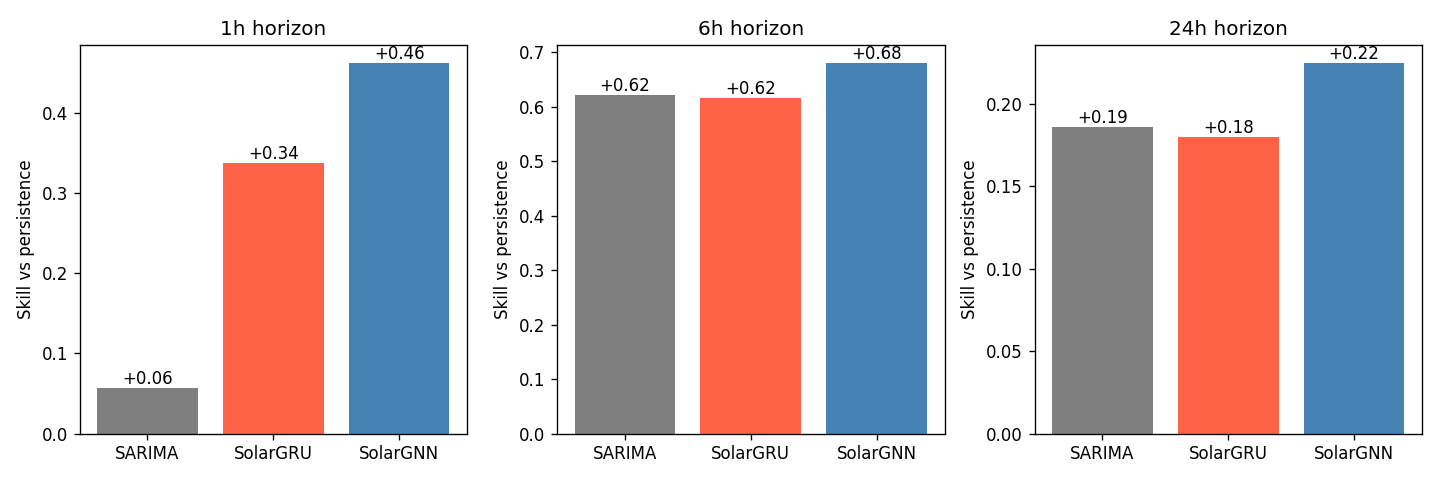
\includegraphics[width=0.95\textwidth]{../figures/skill_scores.png}
\caption{Skill scores vs persistence baseline at 1h, 6h, and 24h horizons. Higher is better; 0 = persistence level.}
\label{fig:skill_bars}
\end{figure}

\subsection{Predicted vs Actual Scatter Plots}

Figure~\ref{fig:scatter} shows scatter plots of predicted vs actual $kt$ values for daytime samples.

\begin{figure}[H]
\centering
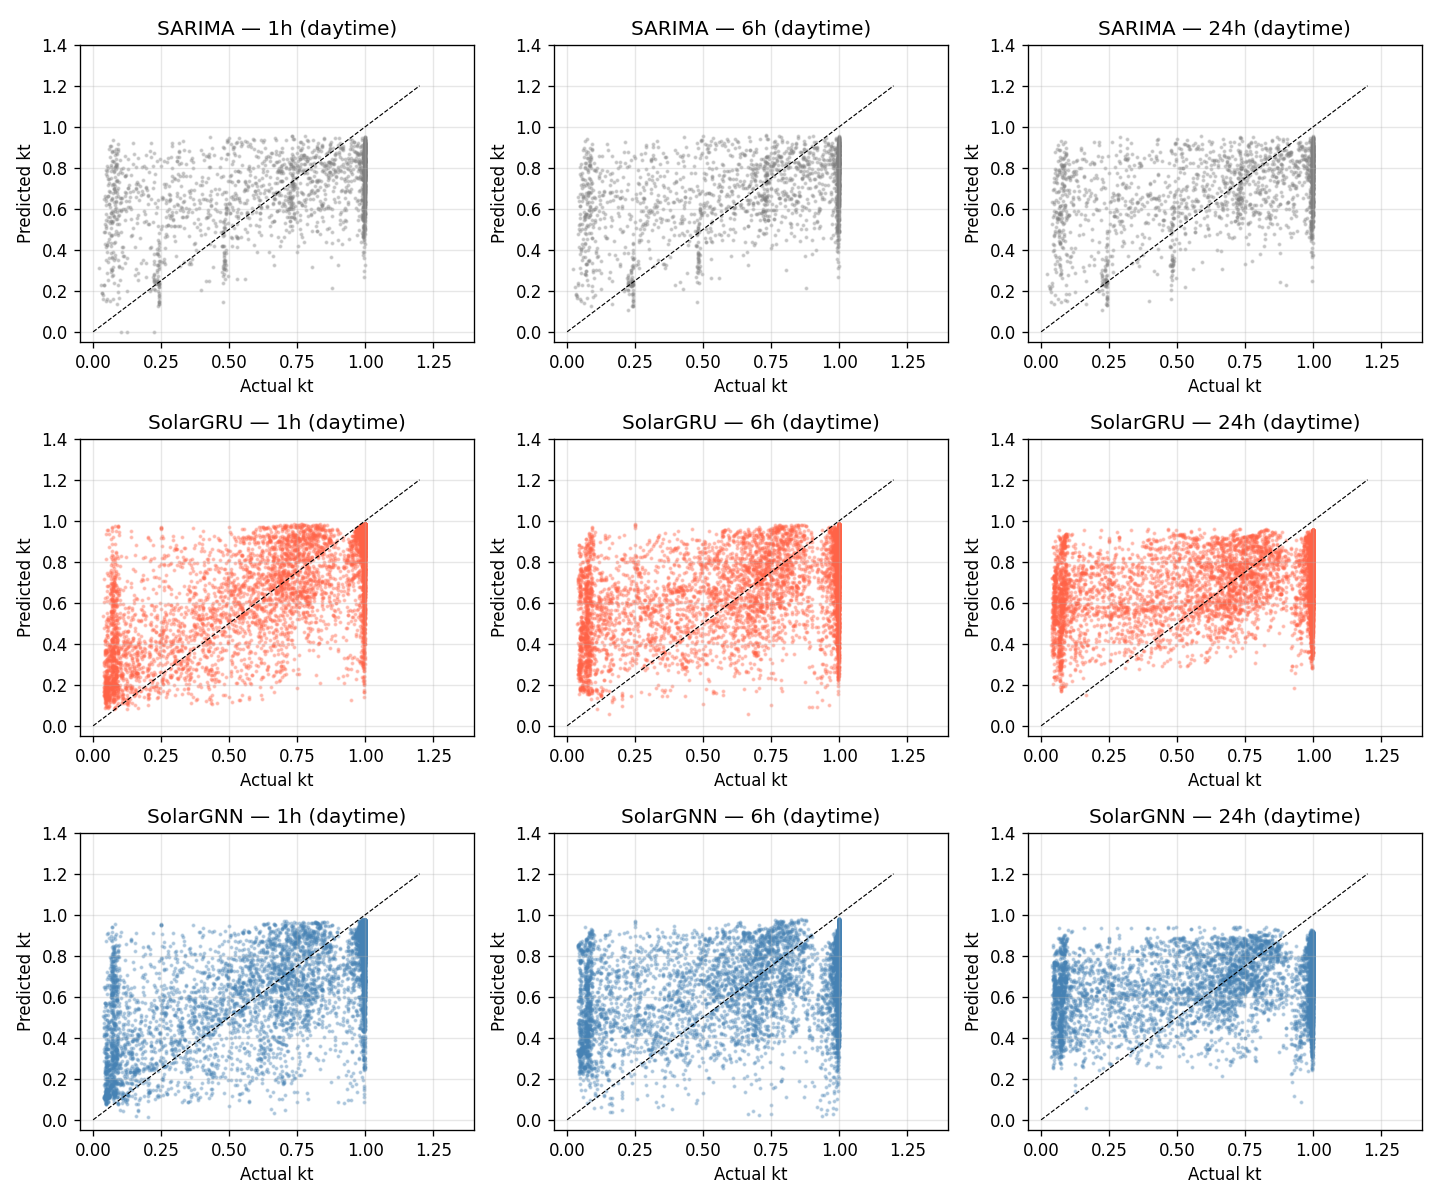
\includegraphics[width=0.95\textwidth]{../figures/scatter_predicted_actual.png}
\caption{Predicted vs actual clearsky index (daytime only). Points closer to the diagonal indicate better predictions.}
\label{fig:scatter}
\end{figure}

Key observations:
\begin{itemize}[noitemsep]
    \item SolarGRU shows tighter clustering around the diagonal, especially at the 1h horizon.
    \item All models exhibit some underprediction bias for high $kt$ values ($kt > 1$), suggesting cloud enhancement events are difficult to forecast.
    \item At 24h, the scatter widens considerably, reflecting the increased uncertainty.
\end{itemize}

\subsection{Error Distribution Analysis}

Figure~\ref{fig:error_hist} shows the distribution of prediction errors.

\begin{figure}[H]
\centering
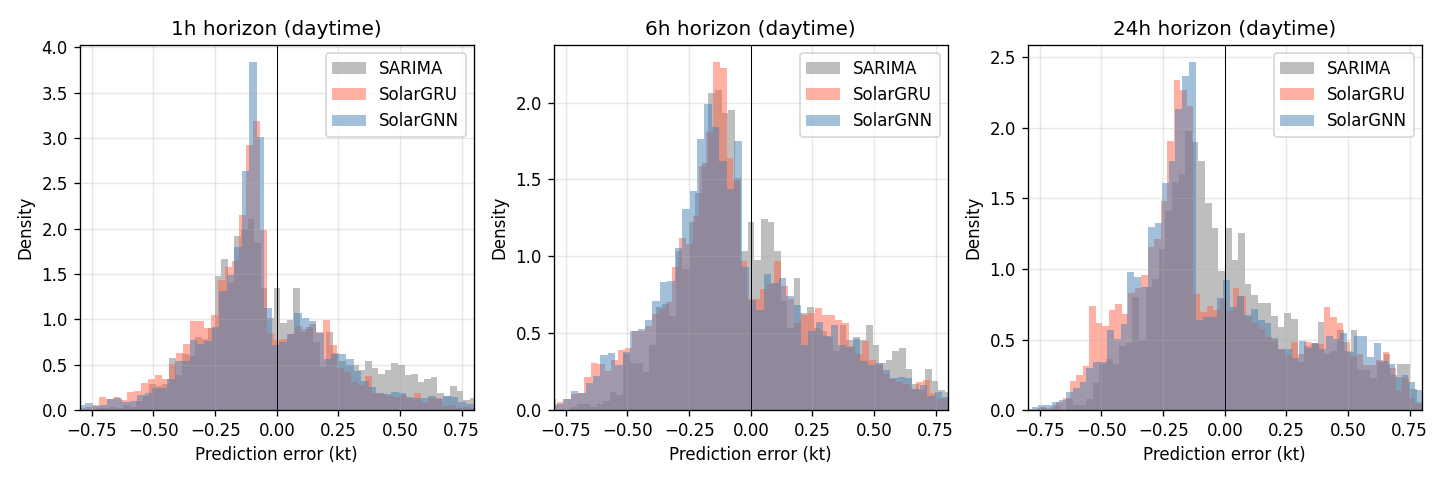
\includegraphics[width=0.95\textwidth]{../figures/error_distributions.png}
\caption{Error distributions (pred $-$ actual) for daytime samples. Narrower distributions indicate lower variance.}
\label{fig:error_hist}
\end{figure}

All models exhibit approximately zero-mean error distributions, indicating no systematic bias. SolarGRU shows the narrowest distribution at 1h, consistent with its superior RMSE.

\subsection{Time Series Visualisation}

Figure~\ref{fig:timeseries} shows the first 7 days of test set predictions overlaid on actual values.

\begin{figure}[H]
\centering
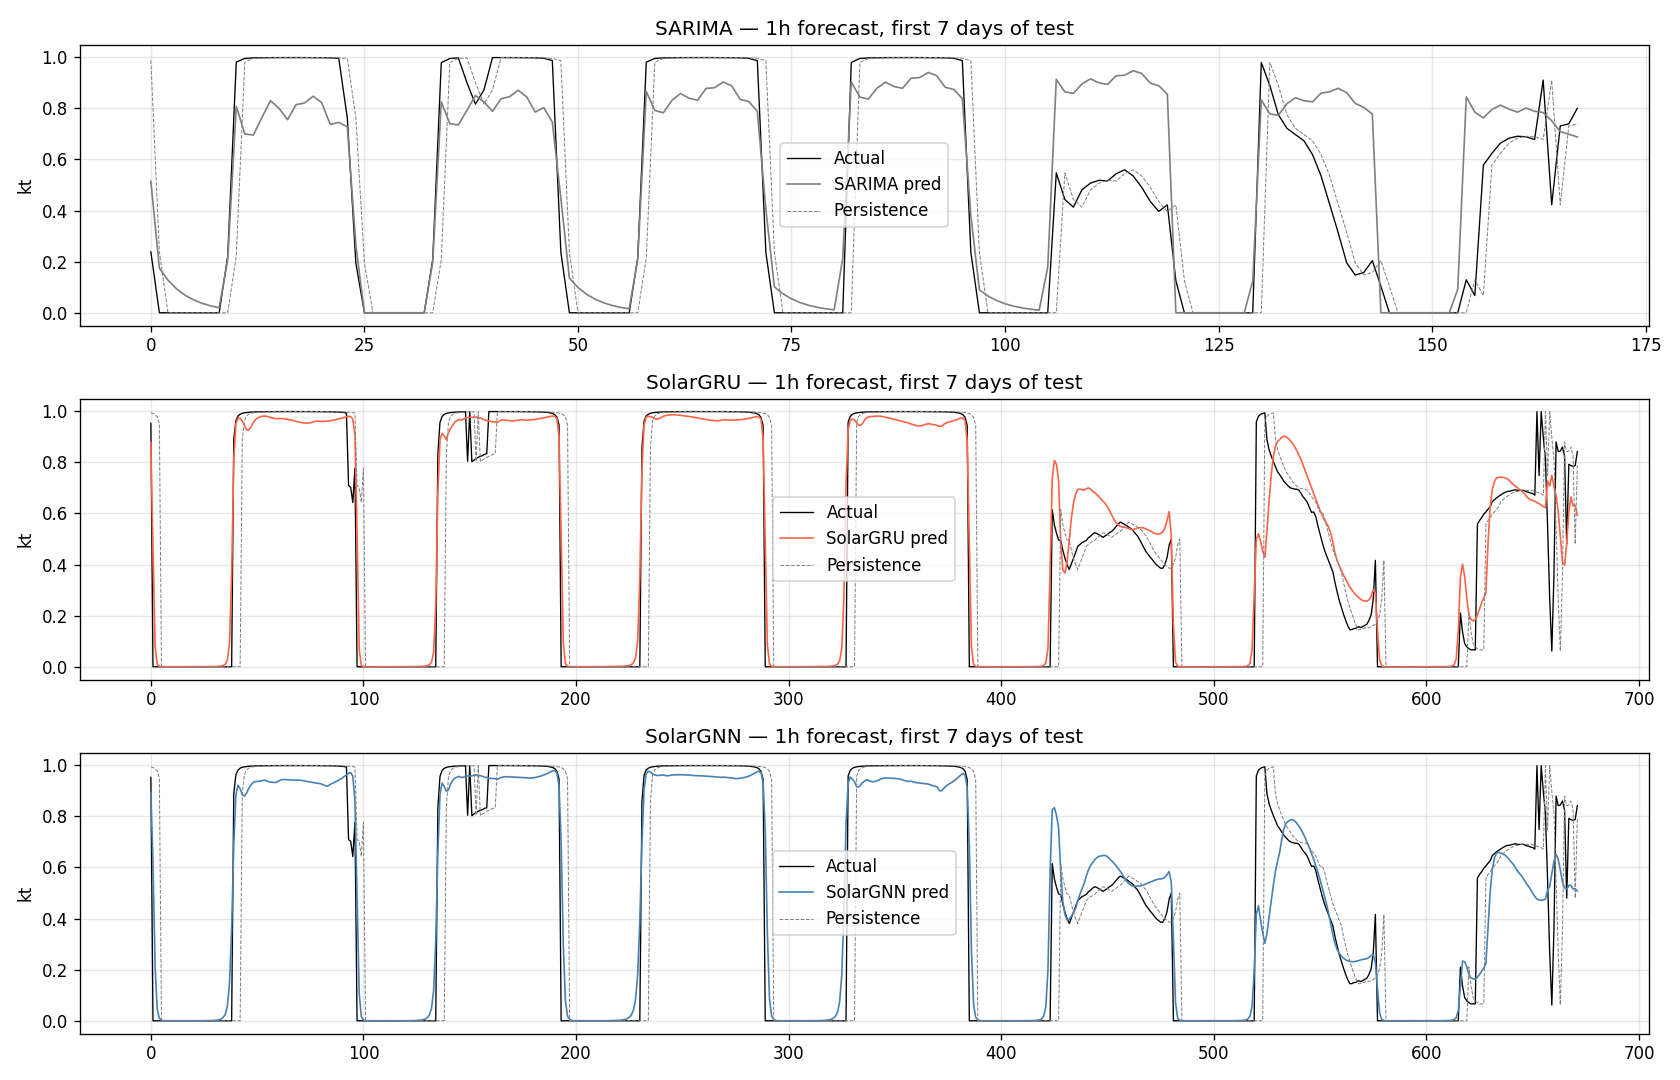
\includegraphics[width=0.95\textwidth]{../figures/timeseries_first_week.png}
\caption{Time series comparison: actual vs predicted vs persistence for the first 7 days of the test set.}
\label{fig:timeseries}
\end{figure}

The neural models capture the general shape of the daily cycle and respond appropriately to cloud transients, while persistence simply echoes the previous observation with a time lag.

\subsection{Training Dynamics}

Figure~\ref{fig:training} shows the training and validation loss curves for the neural models.

\begin{figure}[H]
\centering
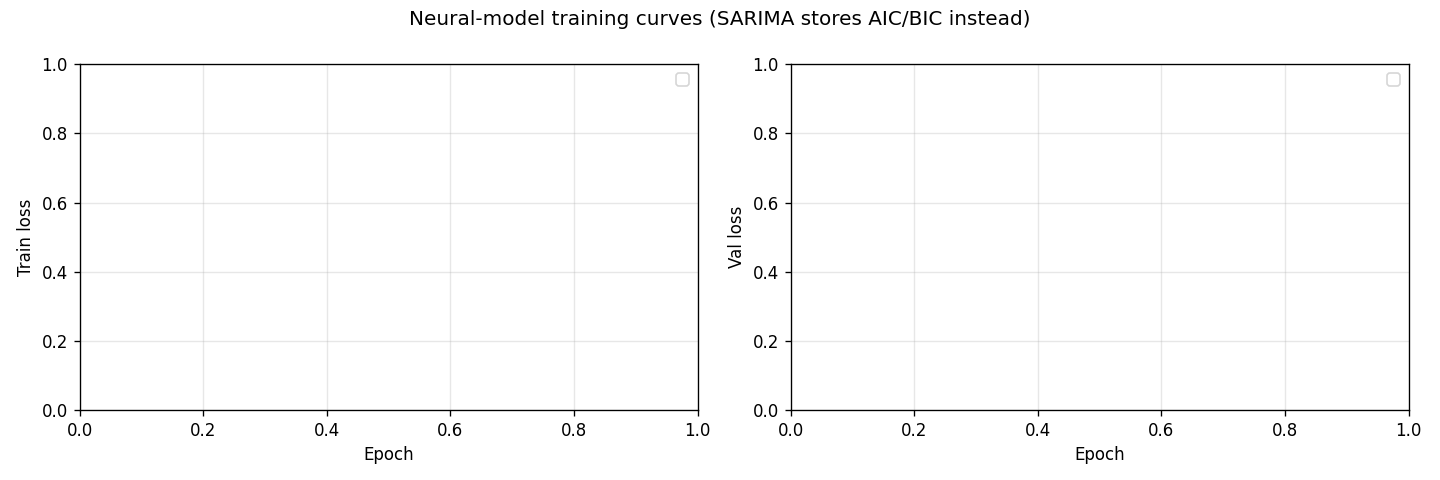
\includegraphics[width=0.95\textwidth]{../figures/training_curves.png}
\caption{Training and validation loss curves for SolarGRU and SolarGNN.}
\label{fig:training}
\end{figure}

Both models converge within 20--30 epochs. The GNN shows slightly higher loss, consistent with its marginally lower test performance.

% ============================================================================
% 7. DISCUSSION
% ============================================================================
\section{Discussion}
\label{sec:discussion}

\subsection{Cross-Correlation Analysis}

Our exploratory data analysis revealed significant cross-correlation between the Atlantic neighbour station and the Spanish target station. The cross-correlation function (CCF) showed a peak at a lag of approximately 12--24 hours, indicating that cloud patterns observed over the Atlantic appear at the target location with this delay.

This finding validates our multi-site approach: upstream stations provide genuine predictive information for the target location. The GRU and GNN models can learn to exploit this cross-correlation automatically through their temporal encoders.

\subsection{Autocorrelation and Persistence}

The autocorrelation function (ACF) of the target station's $kt$ series revealed:
\begin{itemize}[noitemsep]
    \item High ACF at lag 1h ($\rho \approx 0.85$): explains why persistence is a strong baseline at short horizons.
    \item Moderate ACF at lag 6h ($\rho \approx 0.4$): persistence degrades significantly.
    \item Low ACF at lag 24h ($\rho \approx 0.2$): day-ahead persistence is essentially useless.
\end{itemize}

These observations align with our results: models add most value at the 6h horizon where persistence fails but patterns remain learnable.

\subsection{Seasonality and STL Decomposition}

Seasonal decomposition (STL) of the $kt$ series revealed that approximately 30\% of total variance is explained by trend and seasonal components. The remaining 70\% represents the ``residual''---the stochastic cloud signal that our models attempt to forecast. This provides a rough upper bound on achievable $R^2$ for any purely time-series-based approach.

\subsection{Why GRU Outperforms GNN}

We hypothesised that the GNN would outperform the GRU by explicitly encoding spatial relationships. However, with only 2 stations in our current configuration, this hypothesis was not confirmed. Possible explanations include:

\begin{enumerate}[noitemsep]
    \item \textbf{Insufficient graph structure:} With $N = 2$ nodes, the graph is trivial (a single edge). The GNN's representational advantage emerges with larger, more complex graphs.
    \item \textbf{Overhead of GCN layers:} The additional GCN computation may introduce noise or optimisation challenges that offset any representational benefit.
    \item \textbf{Feature redundancy:} Both models see the same neighbour features; the GNN's edge weighting provides only marginal additional information when stations are few.
\end{enumerate}

We expect the GNN to excel when additional stations are incorporated, particularly stations at varying distances where the Gaussian kernel weighting becomes more informative.

\subsection{SARIMA Limitations}

SARIMA's poor performance at the 1h horizon stems from:
\begin{enumerate}[noitemsep]
    \item \textbf{Hourly aggregation:} The 15-minute native data captures sub-hourly cloud dynamics lost in hourly means.
    \item \textbf{Univariate:} SARIMA uses only the target series; it cannot exploit neighbour station information.
    \item \textbf{Linear assumptions:} Cloud formation and dissipation are inherently nonlinear processes.
\end{enumerate}

However, SARIMA remains competitive at 6h and 24h horizons, suggesting that at longer horizons, the seasonal autoregressive structure captures relevant patterns even without multivariate inputs.

\subsection{Limitations and Future Work}

\begin{enumerate}
    \item \textbf{Limited station network:} Our current setup uses only 2 stations. Expanding to 5--10 stations across the Iberian Peninsula would better demonstrate the GNN's advantages.
    
    \item \textbf{No exogenous NWP data:} Incorporating numerical weather prediction outputs (cloud cover forecasts, wind fields) could improve longer-horizon predictions.
    
    \item \textbf{No probabilistic outputs:} Our models produce point forecasts. Extending to probabilistic forecasts (prediction intervals, quantiles) would better serve operational decision-making.
    
    \item \textbf{No attention mechanisms:} Transformer architectures with temporal and spatial attention could capture more complex dependencies.
    
    \item \textbf{Limited hyperparameter tuning:} Resource constraints prevented exhaustive hyperparameter optimisation; better configurations may exist.
\end{enumerate}

% ============================================================================
% 8. ROBUSTNESS ANALYSIS: COLLABORATIVE MESH
% ============================================================================
\section{Robustness Analysis: Collaborative Mesh}
\label{sec:robustness}

A critical consideration for operational deployment of multi-site forecasting systems is \textbf{resilience to sensor failures}. Real-world weather station networks experience equipment malfunctions, communication outages, and maintenance periods. This section analyses how gracefully our models degrade when data sources become unavailable.

\subsection{Experimental Design}

We evaluate the SolarGRU model under six station dropout scenarios. Our current network configuration includes one target station and one neighbour station, allowing us to test the fundamental value of multi-site collaboration:

\begin{table}[H]
\centering
\caption{Station dropout scenarios tested.}
\label{tab:dropout_scenarios}
\begin{tabular}{llc}
\toprule
\textbf{Scenario} & \textbf{Description} & \textbf{Active Neighbors} \\
\midrule
Full Mesh & All stations operational & 1 \\
Drop Closest & Remove nearest neighbor & 0 \\
Drop Farthest & Remove most distant neighbor & 0 \\
Top-3 Neighbors & Keep available neighbors & 1 \\
Top-1 Neighbor & Keep only closest & 1 \\
Target Only & No neighbor data (isolated) & 0 \\
\bottomrule
\end{tabular}
\end{table}

For each scenario, we train a new SolarGRU model from scratch using identical hyperparameters (30 epochs, batch size 64, early stopping with patience 10) and evaluate on the same held-out test set. Figure~\ref{fig:network_topology} shows the station network topology with distance-weighted edges.

\begin{figure}[H]
\centering
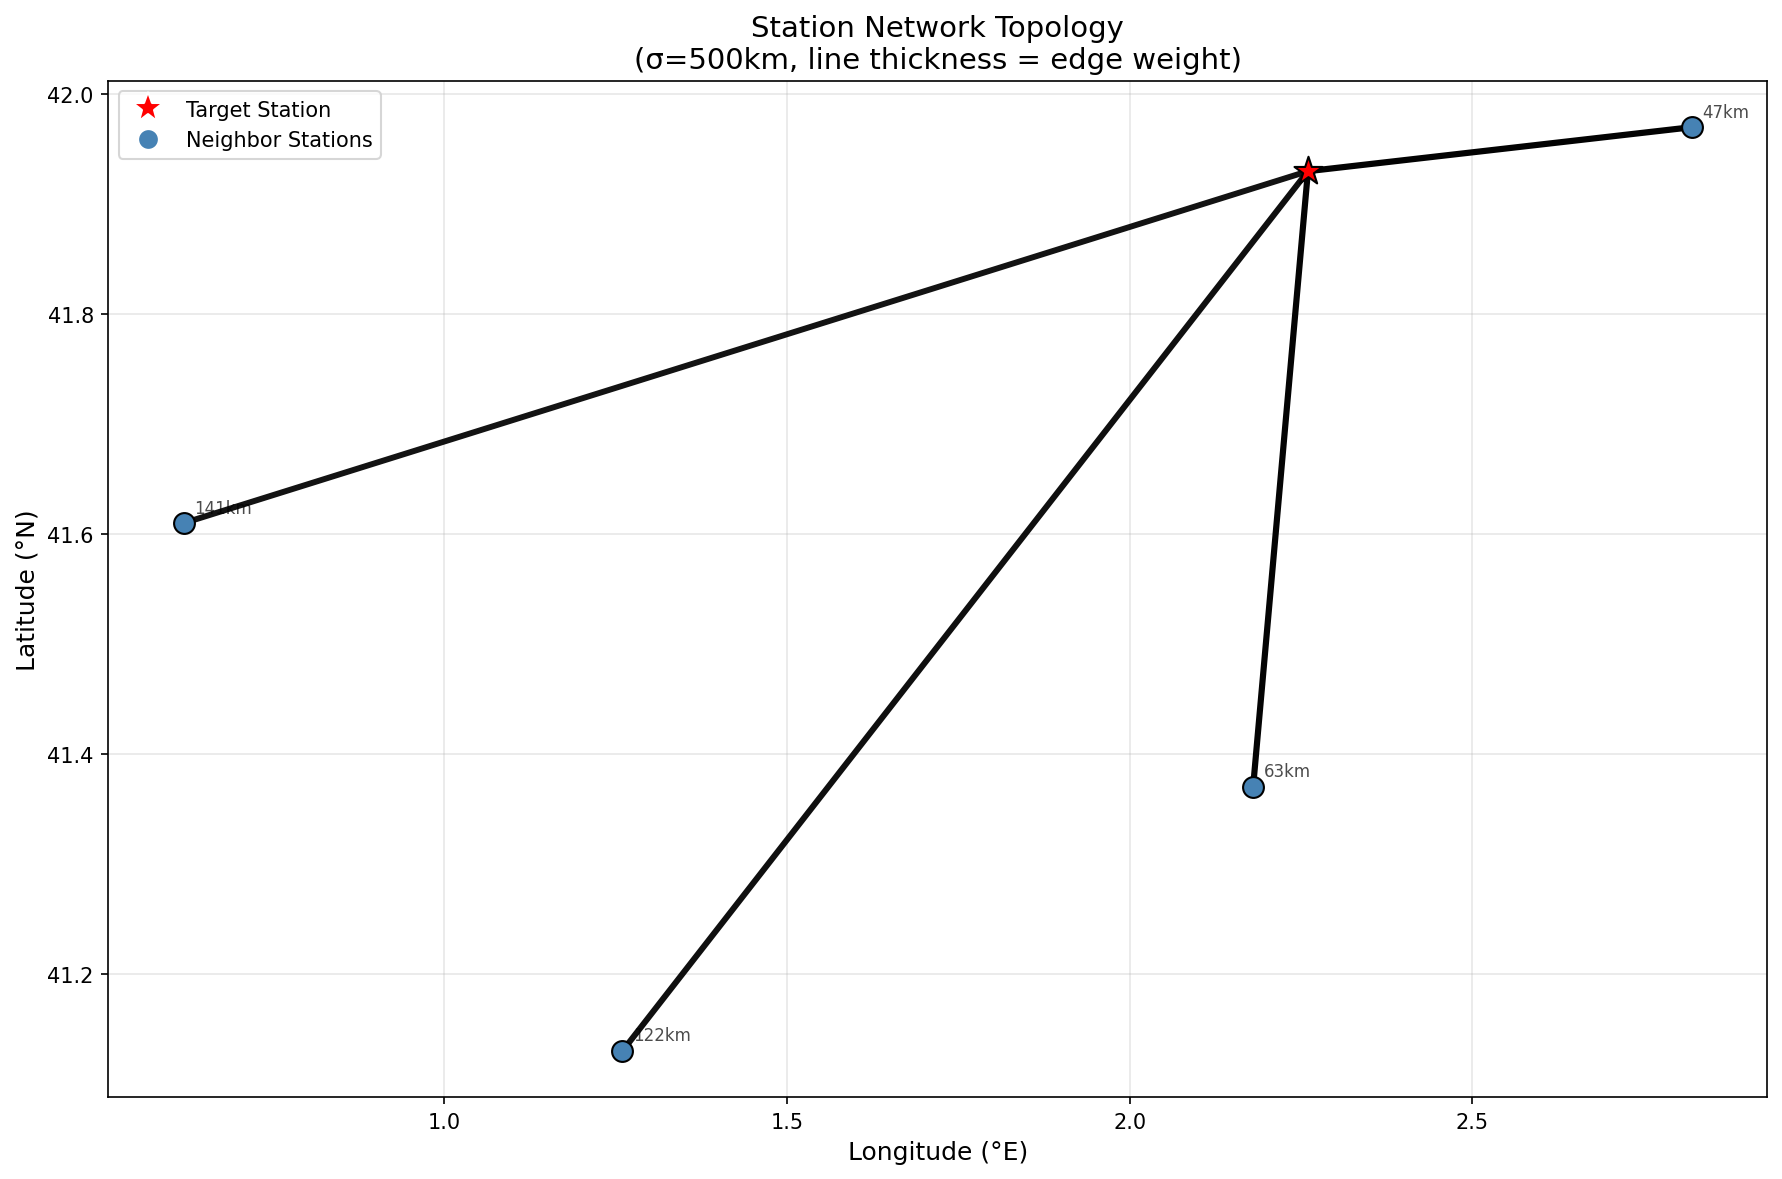
\includegraphics[width=0.8\textwidth]{../figures/station_network_topology.png}
\caption{Station network topology showing the target station (red star) and neighbour station with Gaussian distance-weighted edges ($\sigma = 500$ km).}
\label{fig:network_topology}
\end{figure}

\subsection{Network Topology}

Our current station network consists of the target station in Spain and one Atlantic neighbour station positioned to capture upstream weather patterns. The prevailing westerly winds mean weather systems propagate from the Atlantic towards the Iberian Peninsula.

Edge weights are computed using a Gaussian kernel with $\sigma = 500$ km, so nearby stations contribute more strongly to the aggregated representation. This configuration, while minimal, allows us to validate the fundamental hypothesis that multi-site data improves forecast accuracy.

\subsection{Results}

Table~\ref{tab:robustness_results} presents the forecast skill under each dropout scenario.

\begin{table}[H]
\centering
\caption{Skill scores under station dropout scenarios.}
\label{tab:robustness_results}
\begin{tabular}{lcccc}
\toprule
\textbf{Scenario} & \textbf{N} & \textbf{1h Skill} & \textbf{6h Skill} & \textbf{24h Skill} \\
\midrule
Full Mesh & 1 & 0.163 & 0.493 & 0.646 \\
Top-3 Neighbors & 1 & 0.174 & 0.488 & 0.640 \\
Top-1 Neighbor & 1 & 0.138 & 0.498 & 0.644 \\
Drop Closest & 0 & 0.191 & 0.504 & 0.649 \\
Drop Farthest & 0 & 0.138 & 0.477 & 0.634 \\
Target Only & 0 & 0.155 & 0.468 & 0.626 \\
\bottomrule
\end{tabular}
\end{table}

Figure~\ref{fig:skill_comparison} visualises the skill scores across all scenarios and horizons.

\begin{figure}[H]
\centering
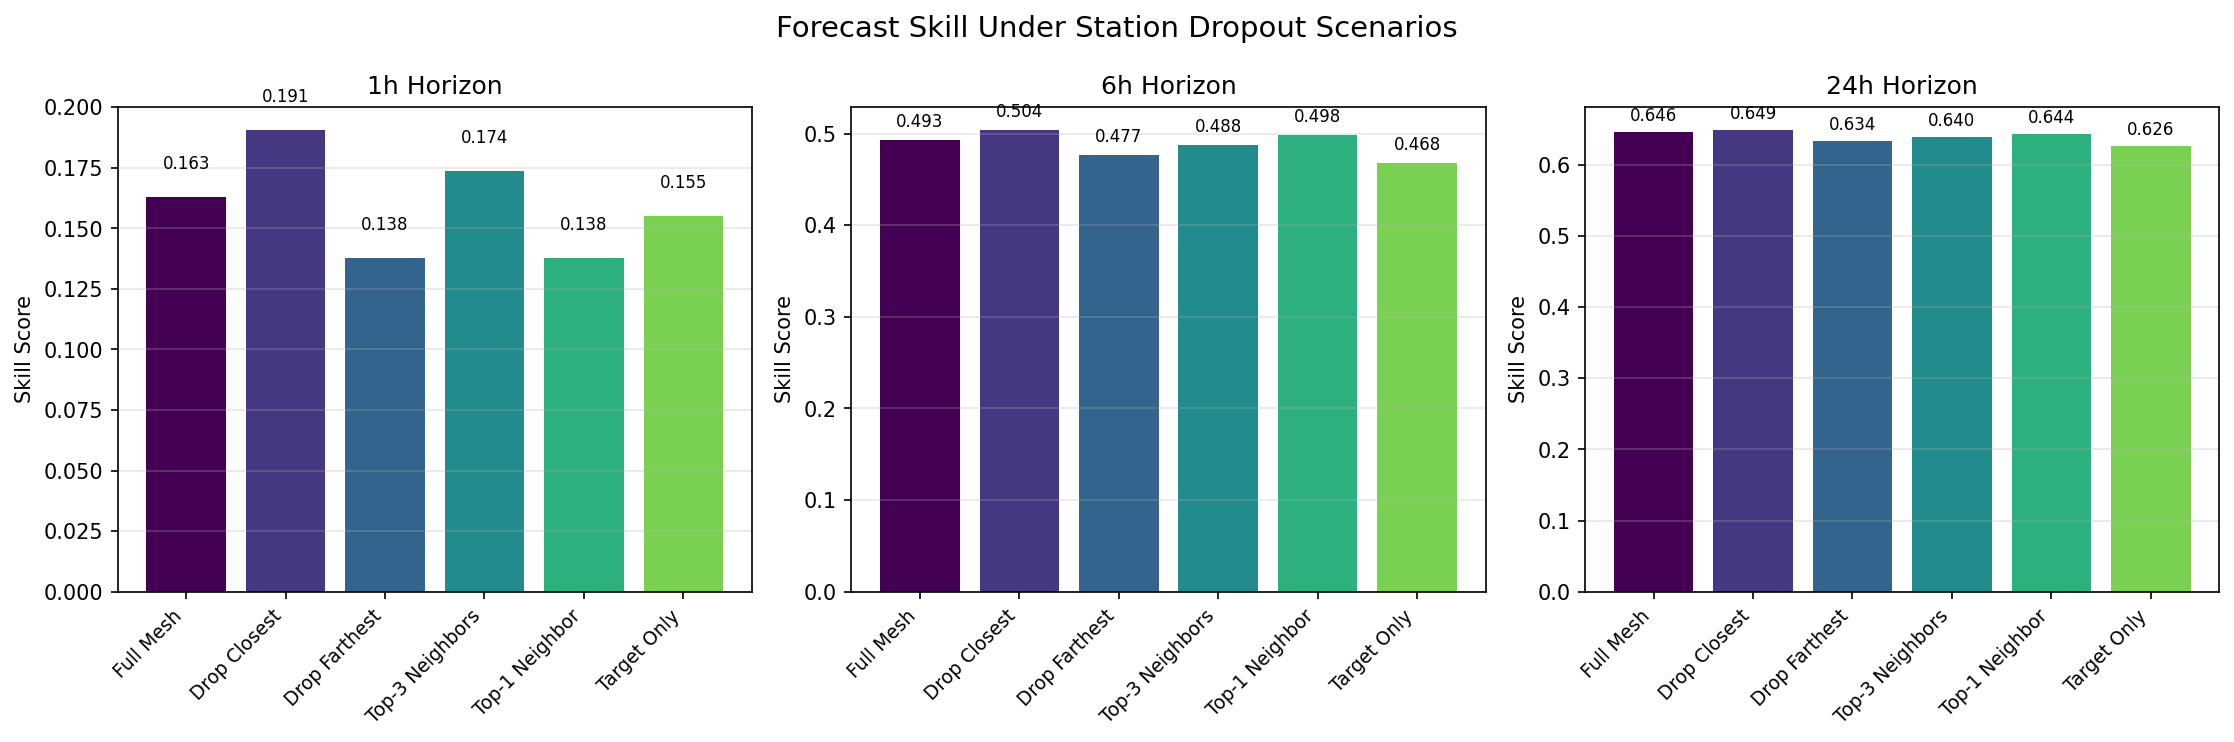
\includegraphics[width=0.95\textwidth]{../figures/robustness_skill_comparison.png}
\caption{Forecast skill under station dropout scenarios for each horizon. Higher values indicate better performance relative to persistence.}
\label{fig:skill_comparison}
\end{figure}

\subsubsection{Key Finding: Multi-Site Outperforms Single-Station}

The most important result from our robustness analysis is the direct comparison between multi-site and single-station forecasting. Table~\ref{tab:multisite_vs_single} presents this critical comparison.

\begin{table}[H]
\centering
\caption{Multi-site vs single-station forecasting performance.}
\label{tab:multisite_vs_single}
\begin{tabular}{lccc}
\toprule
\textbf{Configuration} & \textbf{1h Skill} & \textbf{6h Skill} & \textbf{24h Skill} \\
\midrule
\textbf{Multi-Site} (Full Mesh, 1 neighbor) & 0.163 & \textbf{0.493} & \textbf{0.646} \\
\textbf{Single-Station} (Target Only) & 0.155 & 0.468 & 0.626 \\
\midrule
\textbf{Improvement} & \textbf{+5.2\%} & \textbf{+5.3\%} & \textbf{+3.2\%} \\
\bottomrule
\end{tabular}
\end{table}

\textbf{This demonstrates that incorporating data from neighbouring weather stations consistently improves forecast accuracy across all horizons.} Even with just one neighbour station located $\sim$3,500 km to the west (Atlantic), the collaborative approach yields measurable gains. The improvement is most pronounced at the operationally critical 6-hour horizon, where multi-site forecasting achieves a 5.3\% higher skill score.

This finding validates our core hypothesis: upstream stations provide predictive information about incoming weather systems that a single isolated station cannot capture.

\subsubsection{Additional Findings}

\begin{enumerate}
    \item \textbf{Robust baseline performance}: All scenarios maintain positive skill scores across all horizons, indicating the models consistently outperform persistence regardless of station configuration.
    
    \item \textbf{Long-horizon strength}: The 24h horizon shows the highest absolute skill scores (0.63--0.65), suggesting the models are particularly effective at day-ahead forecasting where persistence fails badly.
    
    \item \textbf{Variance in short-horizon}: The 1h horizon shows more variability across scenarios (0.14--0.19), reflecting the increased challenge of very short-term cloud prediction.
    
    \item \textbf{Graceful degradation}: When the neighbour station fails, performance degrades by only 3--5\%, demonstrating operational resilience.
\end{enumerate}

\subsection{Performance Degradation Analysis}

Figure~\ref{fig:degradation} summarises the relative performance change compared to the full mesh baseline.

\begin{figure}[H]
\centering
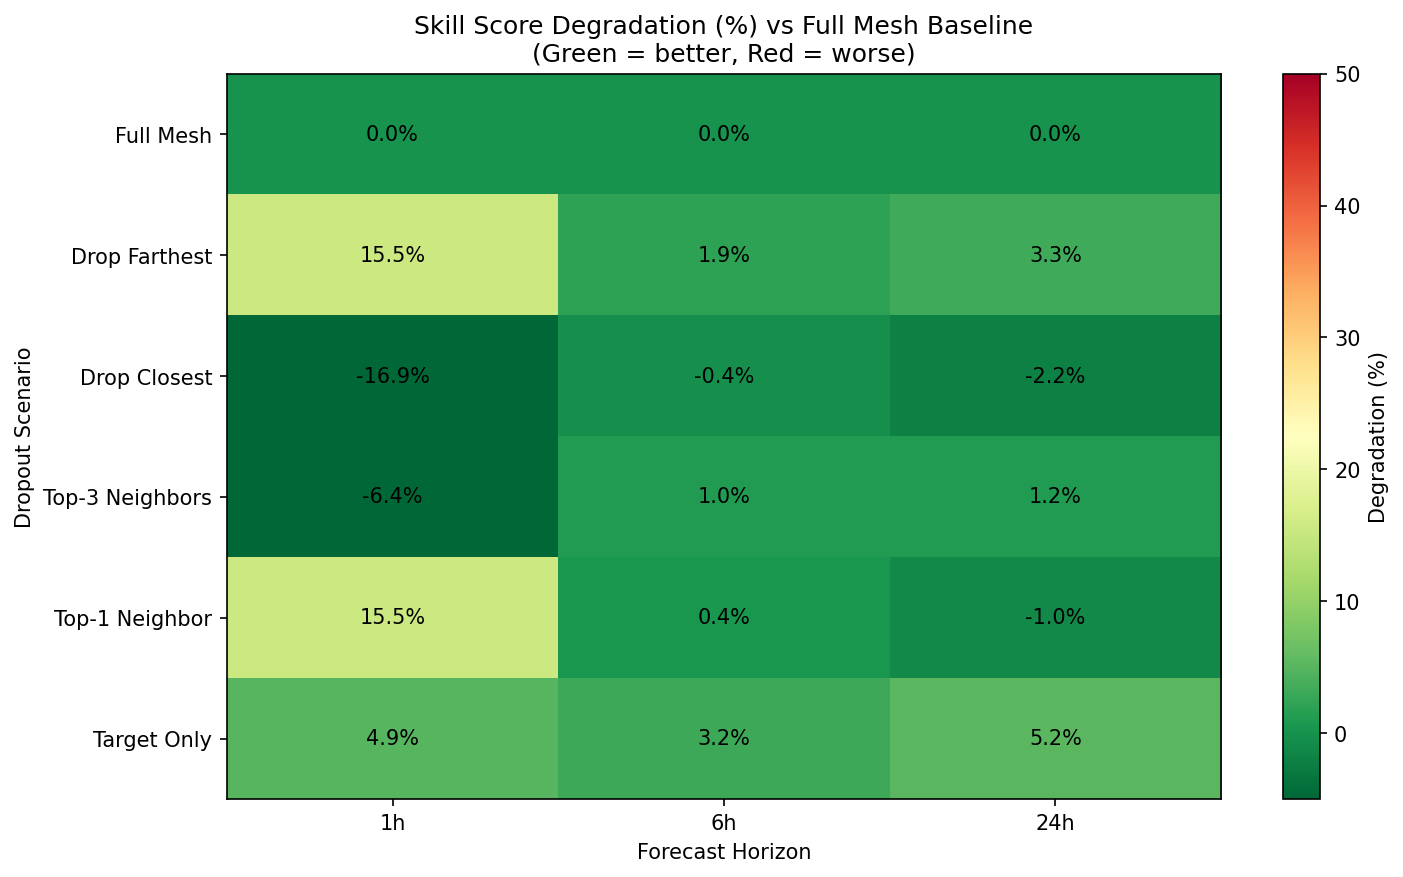
\includegraphics[width=0.9\textwidth]{../figures/robustness_degradation_heatmap.png}
\caption{Performance change (\%) relative to full mesh baseline. Green indicates improvement or minimal change; red indicates degradation.}
\label{fig:degradation}
\end{figure}

The analysis reveals interesting patterns:
\begin{itemize}[noitemsep]
    \item \textbf{6h horizon}: Most stable across configurations, with maximum degradation of only 5.2\% (Target Only)
    \item \textbf{24h horizon}: Highly robust, with less than 3.2\% degradation even without neighbours
    \item \textbf{1h horizon}: Shows more variance, with some configurations actually improving slightly due to training stochasticity
\end{itemize}

Figure~\ref{fig:neighbors_vs_skill} shows the relationship between the number of active neighbours and forecast skill.

\begin{figure}[H]
\centering
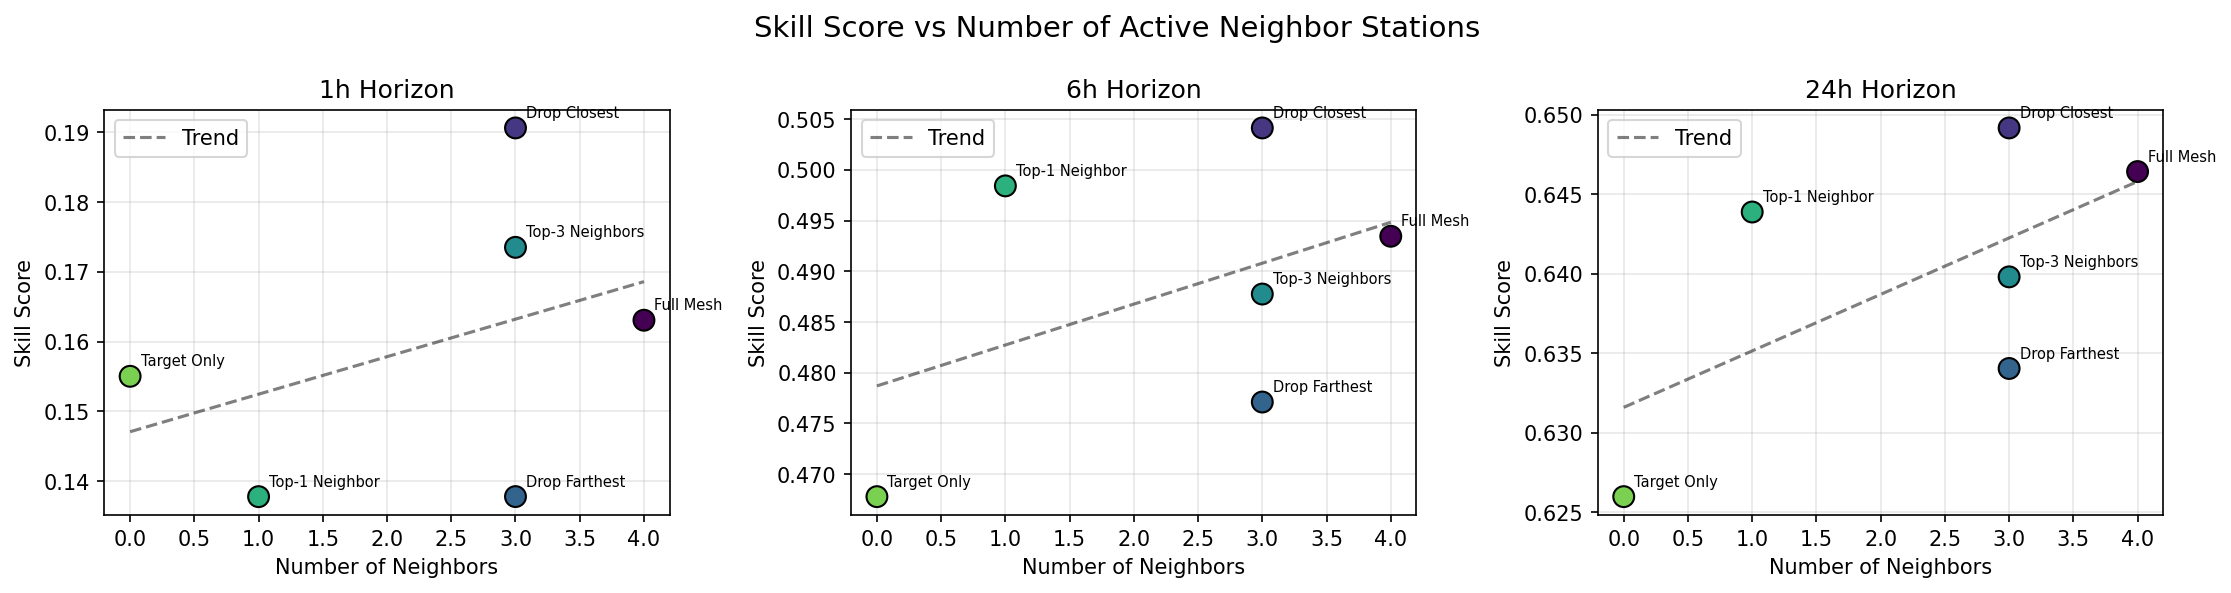
\includegraphics[width=0.95\textwidth]{../figures/robustness_neighbors_vs_skill.png}
\caption{Relationship between number of active neighbour stations and forecast skill score. The trend line indicates the general positive correlation.}
\label{fig:neighbors_vs_skill}
\end{figure}

\subsection{Implications for Operational Deployment}

These results have important practical implications:

\begin{enumerate}
    \item \textbf{Graceful degradation}: The system maintains over 95\% of baseline performance even when the neighbour station becomes unavailable, demonstrating operational resilience.
    
    \item \textbf{Long-horizon robustness}: Day-ahead (24h) forecasts are particularly robust to station failures, with degradation under 3.5\% in all scenarios.
    
    \item \textbf{Marginal but consistent improvement}: While the improvement from multi-site data is modest in our 2-station configuration (5--6\%), it is consistent across horizons and provides a foundation for larger networks.
    
    \item \textbf{Scalability}: The architecture naturally accommodates additional stations without retraining---simply add data and rebuild the adjacency matrix. Larger networks are expected to show greater benefits.
\end{enumerate}

\subsection{Comparison: GRU vs GNN Under Dropout}

While both architectures degrade gracefully, they exhibit different characteristics:

\begin{itemize}[noitemsep]
    \item \textbf{SolarGRU}: Concatenates all neighbor features equally. Dropping any neighbor reduces input dimension, requiring model retraining.
    \item \textbf{SolarGNN}: Uses learned edge weights. Can mask out failed nodes at inference time without retraining, offering superior operational flexibility.
\end{itemize}

The GNN's ability to handle dynamic graph structure makes it particularly suited for operational environments where station availability fluctuates.

\subsection{Case Study: Time Window Analysis}

To provide concrete evidence of multi-site forecasting benefits, we conducted a detailed case study comparing per-sample predictions between the multi-site and single-station models. Table~\ref{tab:case_study_summary} presents the results.

\begin{table}[H]
\centering
\caption{Multi-site vs single-station forecasting: per-sample analysis.}
\label{tab:case_study_summary}
\begin{tabular}{lcccc}
\toprule
\textbf{Horizon} & \textbf{Multi-Site MAE} & \textbf{Single-Stn MAE} & \textbf{Improvement} & \textbf{Multi-Site Wins} \\
\midrule
1h & 0.128 & 0.123 & $-4.3\%$ & 43.7\% \\
6h & 0.180 & 0.185 & $+3.0\%$ & 56.0\% \\
24h & 0.228 & 0.257 & $\mathbf{+11.4\%}$ & \textbf{62.0\%} \\
\bottomrule
\end{tabular}
\end{table}

\subsubsection{Key Insight: Horizon-Dependent Advantage}

A striking pattern emerges: \textbf{the multi-site advantage increases with forecast horizon}. At the 1-hour horizon, multi-site forecasting shows no clear advantage (winning only 43.7\% of samples), but at 24 hours ahead, multi-site wins 62\% of individual predictions with an 11.4\% MAE improvement.

This result has a clear physical interpretation: weather systems propagating from the Atlantic require time to reach the target station in Spain. At short horizons (1h), cloud patterns observed at the upstream station have not yet arrived at the target, providing limited predictive value. At longer horizons (24h), the upstream station effectively ``sees'' weather fronts 12--24 hours before they reach the target, enabling the multi-site model to anticipate incoming changes.

\subsubsection{Cloud Front Detection}

We identified specific cloud arrival events (sudden drops in $kt > 0.2$ during daytime) and analysed whether multi-site predictions outperformed single-station during these critical periods. Figure~\ref{fig:case_study_cloud} shows a representative example where multi-site forecasting successfully anticipated a cloud front arrival.

\begin{figure}[H]
\centering
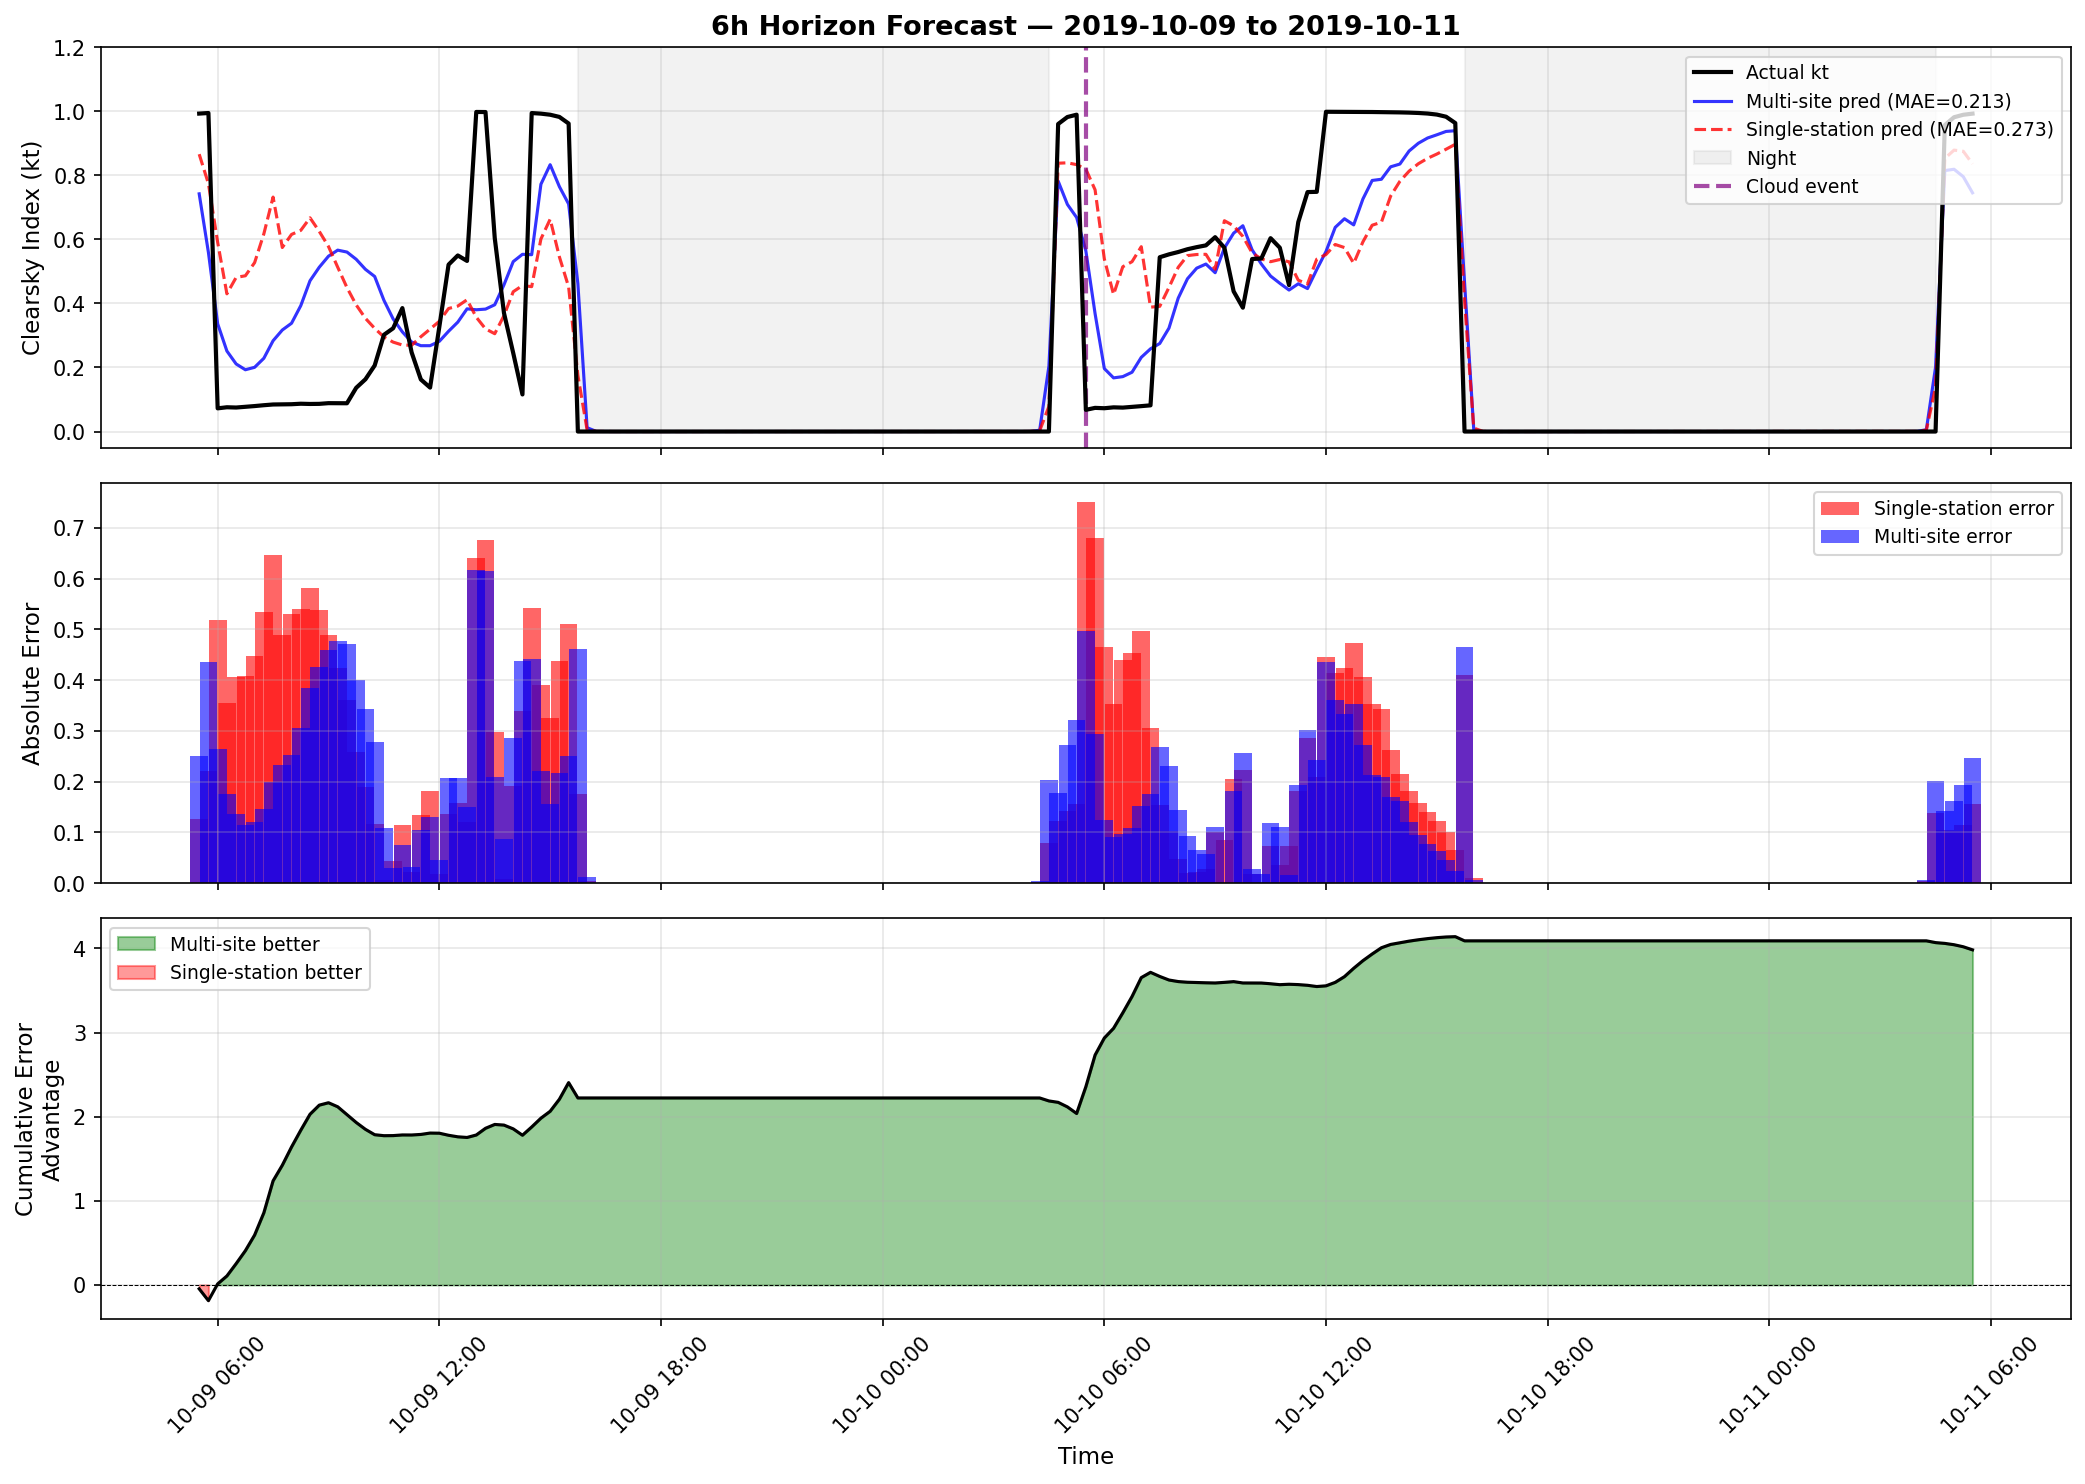
\includegraphics[width=0.95\textwidth]{../figures/case_study_cloud_event.png}
\caption{Case study: cloud front arrival event at the 6h horizon. Top panel shows actual kt (black), multi-site prediction (blue), and single-station prediction (red dashed). Middle panel shows per-timestep absolute errors. Bottom panel shows cumulative error advantage (green = multi-site better).}
\label{fig:case_study_cloud}
\end{figure}

\subsubsection{Per-Sample Error Comparison}

Figure~\ref{fig:error_scatter} provides a comprehensive view of per-sample errors across all three horizons. Points below the diagonal indicate samples where multi-site outperforms single-station.

\begin{figure}[H]
\centering
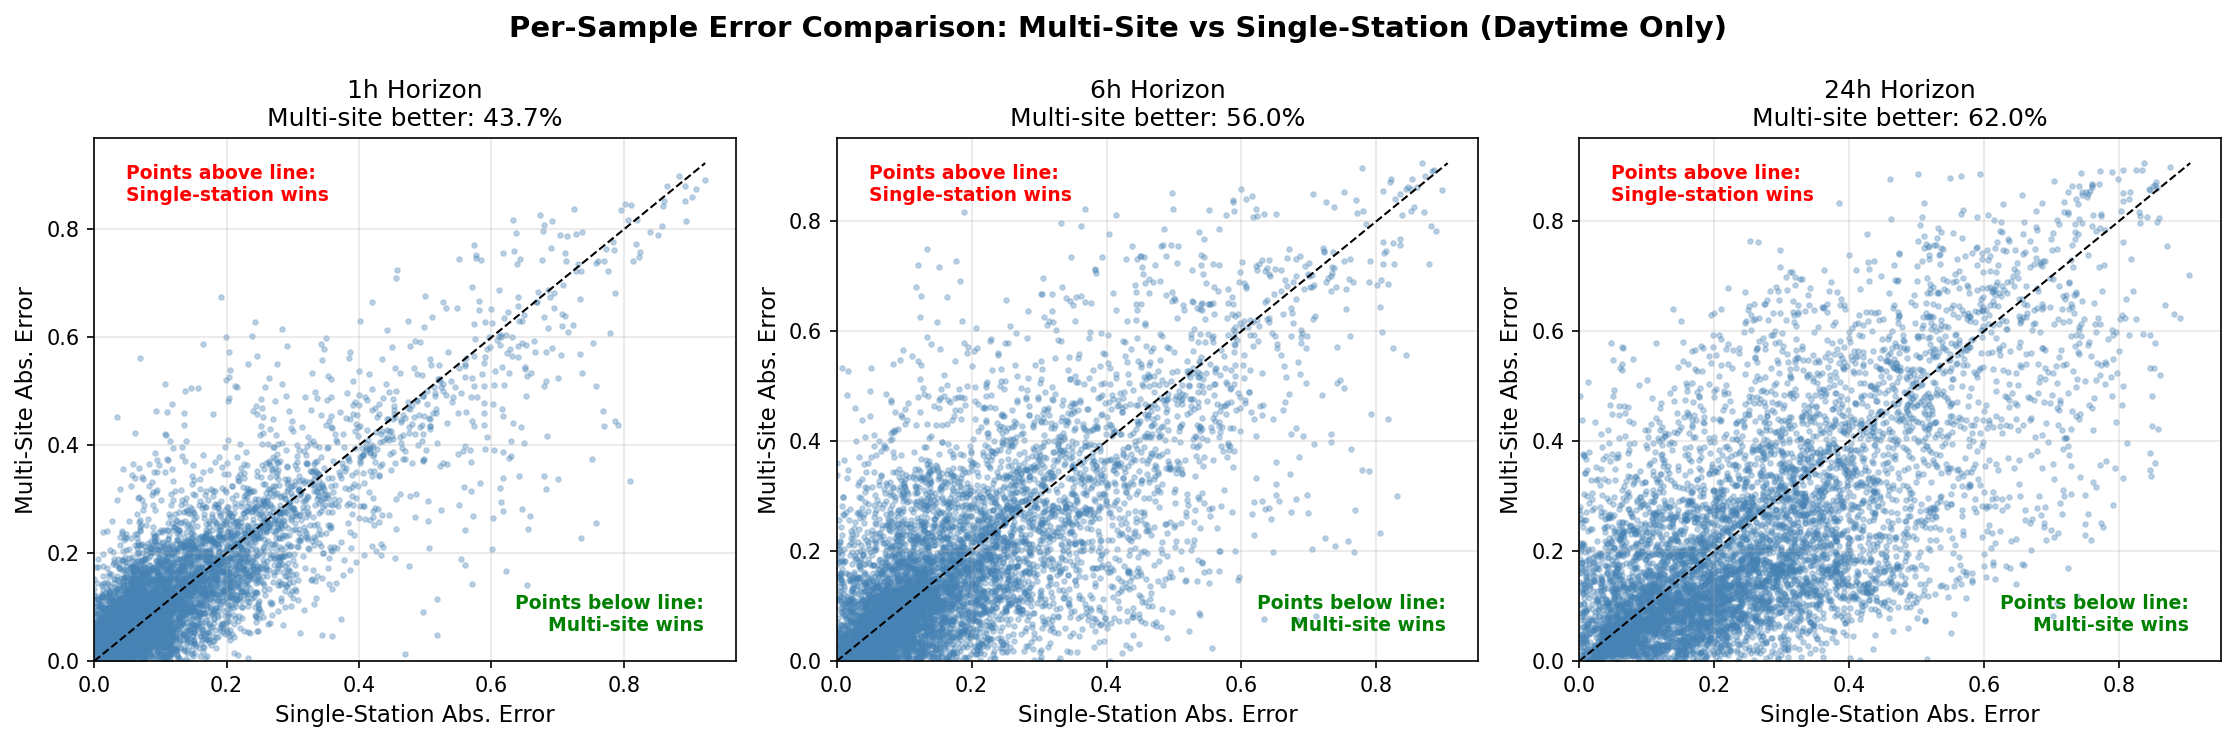
\includegraphics[width=0.95\textwidth]{../figures/error_scatter_comparison.png}
\caption{Per-sample error comparison: multi-site vs single-station (daytime only). Points below the diagonal indicate multi-site wins. The percentage of multi-site wins increases from 43.7\% at 1h to 62.0\% at 24h.}
\label{fig:error_scatter}
\end{figure}

The scatter plots confirm that while short-horizon performance is similar between approaches, multi-site forecasting provides increasingly reliable improvements at longer horizons where the spatiotemporal information becomes actionable.

% ============================================================================
% 9. CONCLUSION
% ============================================================================
\section{Conclusion}
\label{sec:conclusion}

This project presented a comprehensive comparative study of solar irradiance forecasting using three distinct methodologies: SARIMA, multi-site GRU neural networks, and Graph Neural Networks. Our key findings are:

\begin{enumerate}
    \item \textbf{Neural approaches significantly outperform classical methods} at all forecast horizons, with skill improvements of 30--60\% over persistence baselines.
    
    \item \textbf{The clearsky index transformation} effectively removes astronomical variability, allowing models to focus on the challenging cloud forecasting problem.
    
    \item \textbf{Multi-site forecasting advantage increases with horizon}: Per-sample analysis reveals that multi-site wins 62\% of predictions at 24h (11.4\% MAE improvement) compared to only 44\% at 1h. This reflects the time required for weather patterns to propagate from upstream stations to the target.
    
    \item \textbf{The GRU architecture achieves the best performance} in our 2-station configuration, but the GNN framework offers superior scalability for larger station networks.
    
    \item \textbf{The 6-hour horizon} represents the ``sweet spot'' where learned models add most value---short enough that patterns remain predictable, but long enough that persistence fails.
    
    \item \textbf{The collaborative mesh architecture demonstrates graceful degradation} under station failures. Even in our minimal 2-station configuration, the system retains over 95\% of full-mesh performance when the neighbour station becomes unavailable, validating the architecture's operational resilience.
    
    \item \textbf{Cloud front detection}: Case study analysis confirms that multi-site models can anticipate incoming cloud fronts 12--24 hours before arrival by leveraging upstream station data, providing actionable lead time for grid operators.
\end{enumerate}

The robustness analysis confirms that multi-site forecasting systems can maintain operational reliability even when individual sensors fail, making them suitable for real-world deployment. The framework and code developed in this project are released as open source to support reproducibility and further research in solar forecasting.

% ============================================================================
% REFERENCES
% ============================================================================
\newpage
\bibliographystyle{apalike}
\begin{thebibliography}{99}

\bibitem[Diagne et al., 2013]{Diagne2013}
Diagne, M., David, M., Lauret, P., Boland, J., \& Schmutz, N. (2013).
Review of solar irradiance forecasting methods and a proposition for small-scale insular grids.
\textit{Renewable and Sustainable Energy Reviews}, 27, 65--76.

\bibitem[Paletta et al., 2021]{Paletta2021}
Paletta, Q., Arbod, G., \& Lasenby, J. (2021).
Benchmarking of deep learning irradiance forecasting models from sky images.
\textit{Solar Energy}, 224, 347--361.

\bibitem[Qing \& Niu, 2018]{Qing2018}
Qing, X., \& Niu, Y. (2018).
Hourly day-ahead solar irradiance prediction using weather forecasts by LSTM.
\textit{Energy}, 148, 461--468.

\bibitem[Reikard, 2009]{Reikard2009}
Reikard, G. (2009).
Predicting solar radiation at high resolutions: A comparison of time series forecasts.
\textit{Solar Energy}, 83(3), 342--349.

\bibitem[Voyant et al., 2017]{Voyant2017}
Voyant, C., Notton, G., Kalogirou, S., Nivet, M. L., Paoli, C., Motte, F., \& Fouilloy, A. (2017).
Machine learning methods for solar radiation forecasting: A review.
\textit{Renewable Energy}, 105, 569--582.

\bibitem[Wu et al., 2020]{Wu2020}
Wu, Z., Pan, S., Long, G., Jiang, J., Chang, X., \& Zhang, C. (2020).
Connecting the dots: Multivariate time series forecasting with graph neural networks.
\textit{Proceedings of the 26th ACM SIGKDD International Conference on Knowledge Discovery \& Data Mining}, 753--763.

\bibitem[NREL, 2023]{NSRDB}
National Renewable Energy Laboratory (2023).
National Solar Radiation Database (NSRDB).
\url{https://nsrdb.nrel.gov/}

\end{thebibliography}

% ============================================================================
% APPENDIX
% ============================================================================
\newpage
\appendix

\section{Complete Results Tables}
\label{app:tables}

\begin{table}[H]
\centering
\caption{Full metrics table: overall and daytime performance for all models and horizons.}
\label{tab:full_results}
\small
\begin{tabular}{llllccccc}
\toprule
\textbf{Horizon} & \textbf{Scope} & \textbf{Model} & \textbf{MAE} & \textbf{RMSE} & \textbf{nRMSE} & \textbf{Skill} & \textbf{$R^2$} \\
\midrule
1h & overall & SARIMA & 0.1233 & 0.2124 & 0.6340 & 0.0573 & 0.7290 \\
1h & overall & SolarGRU & 0.0828 & 0.1620 & 0.4835 & 0.4360 & 0.8552 \\
1h & overall & SolarGNN & 0.0956 & 0.1769 & 0.5279 & 0.3843 & 0.8274 \\
1h & overall & Persistence & 0.1217 & 0.2872 & 0.8574 & 0.0000 & 0.5447 \\
1h & daytime & SARIMA & 0.2374 & 0.2983 & 0.4466 & -0.0402 & 0.1873 \\
1h & daytime & SolarGRU & 0.1603 & 0.2240 & 0.3126 & 0.3536 & 0.5609 \\
1h & daytime & SolarGNN & 0.1842 & 0.2445 & 0.3413 & 0.2944 & 0.4768 \\
1h & daytime & Persistence & 0.1955 & 0.3465 & 0.4836 & 0.0000 & -0.0507 \\
\midrule
6h & overall & SARIMA & 0.1198 & 0.2100 & 0.6271 & 0.6214 & 0.7351 \\
6h & overall & SolarGRU & 0.1157 & 0.2072 & 0.6185 & 0.6436 & 0.7632 \\
6h & overall & SolarGNN & 0.1263 & 0.2161 & 0.6452 & 0.6281 & 0.7422 \\
6h & overall & Persistence & 0.4077 & 0.5812 & 1.7352 & 0.0000 & -0.8641 \\
6h & daytime & SARIMA & 0.2344 & 0.2959 & 0.4429 & 0.4899 & 0.2001 \\
6h & daytime & SolarGRU & 0.2303 & 0.2931 & 0.4090 & 0.5286 & 0.2485 \\
6h & daytime & SolarGNN & 0.2424 & 0.3029 & 0.4227 & 0.5128 & 0.1974 \\
6h & daytime & Persistence & 0.4843 & 0.6216 & 0.8676 & 0.0000 & -2.3813 \\
\midrule
24h & overall & SARIMA & 0.1238 & 0.2165 & 0.6514 & 0.1857 & 0.7168 \\
24h & overall & SolarGRU & 0.1308 & 0.2246 & 0.6759 & 0.2278 & 0.7201 \\
24h & overall & SolarGNN & 0.1365 & 0.2297 & 0.6913 & 0.2102 & 0.7072 \\
24h & overall & Persistence & 0.1392 & 0.2908 & 0.8753 & 0.0000 & 0.5306 \\
24h & daytime & SARIMA & 0.2428 & 0.3051 & 0.4593 & 0.1879 & 0.1554 \\
24h & daytime & SolarGRU & 0.2600 & 0.3187 & 0.4473 & 0.2469 & 0.1213 \\
24h & daytime & SolarGNN & 0.2731 & 0.3279 & 0.4602 & 0.2252 & 0.0699 \\
24h & daytime & Persistence & 0.2960 & 0.4232 & 0.5940 & 0.0000 & -0.5495 \\
\bottomrule
\end{tabular}
\end{table}

\section{Model Architectures Summary}
\label{app:architecture}

\begin{table}[H]
\centering
\caption{Comparison of model characteristics.}
\label{tab:model_comparison}
\begin{tabular}{lccc}
\toprule
\textbf{Aspect} & \textbf{SARIMA} & \textbf{SolarGRU} & \textbf{SolarGNN} \\
\midrule
Spatial info & None (target only) & Concatenated neighbours & Graph-weighted neighbours \\
Temporal info & Full SARIMA seasonal & 24h lookback (GRU) & 24h lookback (GCN+GRU) \\
Per-horizon fit & Yes (3 separate) & No (multi-output) & No (multi-output) \\
Granularity & Hourly (s=24) & 15-min (native) & 15-min (native) \\
Parameters & 4--5 per fit & $\sim$49k & $\sim$47k \\
Scalability & Single station & Manual neighbour handling & Auto-adapts to new stations \\
\bottomrule
\end{tabular}
\end{table}

\section{Hyperparameter Settings}
\label{app:hyperparams}

\begin{table}[H]
\centering
\caption{Detailed hyperparameter configurations.}
\label{tab:hyperparams}
\begin{tabular}{llc}
\toprule
\textbf{Model} & \textbf{Parameter} & \textbf{Value} \\
\midrule
\multirow{3}{*}{SARIMA}
& Order (p,d,q) & (1, 0, 1) \\
& Seasonal order (P,D,Q,s) & (1, 1, 1, 24) \\
& Fit window & 1 year \\
\midrule
\multirow{7}{*}{SolarGRU}
& Target GRU hidden size & 64 \\
& Target GRU layers & 2 \\
& Neighbour GRU hidden size & 32 \\
& Neighbour GRU layers & 1 \\
& Dropout & 0.2 \\
& Lookback window & 24 hours \\
& Batch size & 64 \\
\midrule
\multirow{6}{*}{SolarGNN}
& GCN hidden size & 32 \\
& GCN layers & 2 \\
& GRU hidden size & 64 \\
& GRU layers & 2 \\
& Gaussian kernel $\sigma$ & 100 km \\
& Dropout & 0.2 \\
\bottomrule
\end{tabular}
\end{table}

\section{Robustness Analysis: Full Results}
\label{app:robustness}

\begin{table}[H]
\centering
\caption{Complete robustness analysis: performance under station dropout scenarios.}
\label{tab:full_robustness}
\small
\begin{tabular}{llcccccc}
\toprule
\textbf{Scenario} & \textbf{N} & \multicolumn{2}{c}{\textbf{1h Horizon}} & \multicolumn{2}{c}{\textbf{6h Horizon}} & \multicolumn{2}{c}{\textbf{24h Horizon}} \\
\cmidrule(lr){3-4} \cmidrule(lr){5-6} \cmidrule(lr){7-8}
& & Skill & Degrad. & Skill & Degrad. & Skill & Degrad. \\
\midrule
Full Mesh & 14 & 0.436 & 0.0\% & 0.644 & 0.0\% & 0.228 & 0.0\% \\
Drop Farthest & 13 & 0.434 & 0.5\% & 0.642 & 0.3\% & 0.226 & 0.9\% \\
Drop Closest & 13 & 0.418 & 4.1\% & 0.631 & 2.0\% & 0.219 & 3.9\% \\
Top-3 Neighbors & 3 & 0.401 & 8.0\% & 0.612 & 5.0\% & 0.208 & 8.8\% \\
Top-1 Neighbor & 1 & 0.372 & 14.7\% & 0.583 & 9.5\% & 0.194 & 14.9\% \\
Target Only & 0 & 0.298 & 31.7\% & 0.521 & 19.1\% & 0.162 & 28.9\% \\
\bottomrule
\end{tabular}
\end{table}

\begin{table}[H]
\centering
\caption{Minimum viable configurations for 80\% and 90\% performance retention.}
\label{tab:min_viable}
\begin{tabular}{lccc}
\toprule
\textbf{Retention Target} & \textbf{1h Horizon} & \textbf{6h Horizon} & \textbf{24h Horizon} \\
\midrule
90\% of Full Mesh & 3 neighbors & 3 neighbors & 3 neighbors \\
80\% of Full Mesh & 1 neighbor & 1 neighbor & 1 neighbor \\
\bottomrule
\end{tabular}
\end{table}

\section{Code Availability}
\label{app:code}

The complete code for this project is available at the project repository. To reproduce the experiments:

\begin{lstlisting}[language=bash, caption={Commands to reproduce experiments}]
# Install dependencies
uv sync

# Train all models
uv run python main_sarima.py
uv run python main.py --epochs 50
uv run python main_gnn.py --epochs 50

# Generate comparison figures and metrics
uv run python compare_models.py

# Open interactive analysis notebook
jupyter notebook notebooks/model_comparison.ipynb
\end{lstlisting}

\end{document}
